\documentclass[11pt]{exam}
\usepackage[utf8]{inputenc}
\usepackage[a4paper,top=2cm,left=2cm,right=2cm,bottom=2cm]{geometry}
\usepackage{import}
\usepackage[T1]{fontenc}
\usepackage[german,ngerman]{babel}
\usepackage[table]{xcolor}
\usepackage{amsthm, esvect}
\usepackage{mathtools}
\RequirePackage{amssymb, amsfonts, amsmath, latexsym, verbatim, xspace}
\usepackage{systeme}
\usepackage{multicol}
\usepackage{multirow}
\usepackage{framed}
\usepackage{array}
\usepackage{ragged2e}
\usepackage{graphicx}
\usepackage{pdflscape}
\usepackage{epstopdf}
\usepackage{booktabs}
\usepackage{pdfpages}
\usepackage{float} % Allows putting an [H] in \begin{figure} to specify the exact location of the figure
\usepackage{wrapfig} % Allows in-line images such as the example fish picture
\usepackage{tikz, graphicx} % tikz
\usepackage[position=top]{subfig}
\usepackage[bookmarks=true]{hyperref}%Links
\usepackage{enumerate}
\usepackage{enumitem}
\usepackage[german,ruled,vlined,linesnumbered,algosection]{algorithm2e}
\usepackage[labelfont=sf]{caption}
\usepackage{lmodern}
\usepackage{lscape}
\usepackage{tabularx}
\usepackage{systeme}
\usepackage{hhline}
\usepackage{subfiles}
\usepackage{stackengine}
\usepackage{setspace}
\usepackage{MnSymbol}
\usepackage{tcolorbox}
\usepackage{bbm}
\usepackage{url}
\usepackage{xparse}
\usepackage{sectsty}
\usepackage{array}
\usepackage{ragged2e}
\usepackage{listings} %Stellt Code-Snippets sauber dar

% definiert die Sprache
\selectlanguage{German}

% add command for different dates in Swiss fashion
\newcommand{\monthwordlong}[1]{\ifcase#1 \or Januar\or Februar\or März\or April\or Mai\or Juni\or Juli\or August\or September\or Oktober\or November\or Dezember\fi}
\newcommand{\monthwordshort}[1]{\ifcase#1\or Jan\or Feb\or Mar\or Apr\or Mai\or Jun\or Jul\or Aug\or Sept\or Okt\or Nov\or Dez\fi}
\newcommand{\datelong}{\number\day.\:\monthwordlong{\the\month}\:\number\year}
\newcommand{\dateshort}{\number\day.\:\monthwordshort{\the\month}\:\number\year}

% define color of links inside a text
\definecolor{linkblue}{RGB}{0, 0, 80}
\definecolor{plotblue}{RGB}{100, 100, 255}
\definecolor{myblue}{RGB}{8,164,214}
\definecolor{myred}{RGB}{143,42,41}
\definecolor{forestgreen}{RGB}{34,139,34}
\definecolor{highdive}{RGB}{10,169,194}
\definecolor{charcoal}{RGB}{74,74,74}
\hypersetup{
	colorlinks=true,
	linkcolor=linkblue,
	filecolor=magenta,
	urlcolor=plotblue,
	citecolor=linkblue,
	pdfpagemode=FullScreen,
}


\lstdefinestyle{mystyle}{ % definiert den style des Code-Snippets
	%backgroundcolor=\color{backcolour},
	%commentstyle=\color{codegreen},
	%keywordstyle=\color{magenta},
	%numberstyle=\tiny\color{codegray},
	%stringstyle=\color{codepurple},
	basicstyle=\ttfamily\footnotesize,
	breakatwhitespace=false,
	breaklines=true,
	captionpos=b,
	keepspaces=true,
	%numbers=left,
	%numbersep=5pt,
	showspaces=false,
	showstringspaces=false,
	showtabs=false,
	tabsize=4
}
\lstset{style=mystyle}
\qformat{\Large\textbf{Aufgabe \thequestion\hfill\thepoints}}
\newlist{partes}{enumerate}{3}
\setlist[partes]{label=(\alph*)}
\newcommand{\parte}{\item}
\newlist{subpartes}{enumerate}{3}
\setlist[subpartes]{label=\roman*)}
\newcommand{\subparte}{\item}
\setlist[enumerate,1]{%(
	leftmargin=*, itemsep=12pt, label={\textbf{\arabic*.)}}}
\newcommand\answerbox{%%
	\fbox{\rule{2in}{0pt}\rule[-0.1ex]{0pt}{4ex}}}
\pointpoints{Punkt}{Punkte}
\hqword{Frage:}
\hpword{Mögliche Punkte:}
\hsword{Erreicht:}
\htword{Total}
\renewcommand*\half{.5}
\renewcommand{\solutiontitle}{\noindent\textbf{Lösung:}\par\noindent}

% Graphed boxes
\newcommand{\karos}[2]{
  \begin{tikzpicture}
    \draw[step=0.4cm,color=cyan,dotted] (0,0) grid (#1 cm ,#2 cm);
  %  \draw((#1)/2 cm,0)--((#1)/2 cm,/#2)/2cm)
  \end{tikzpicture}
}
\usetikzlibrary{arrows, petri, topaths, graphs}
\linespread{1.2} % Line spacing

%=========================================================
\newenvironment{parcols}[1][]{
    \begin{parts}\begin{multicols}{#1}
}{
    \end{multicols}\end{parts}
}
%=========================================================
\newenvironment{itemcols}[1][]{
	\begin{itemize}\begin{multicols}{#1}
		}{
	\end{multicols}\end{itemize}
}

%=========================================================
\newcommand{\antwort}[1]{
	{\setlength{\textwidth}{\textwidth}\fillwithgrid{#1cm}\vspace{5pt}}
}

%=========================================================
% Karriertes Papier für Antwort MIT OVERLAY
\tcbuselibrary{breakable,skins}
\usetikzlibrary{mindmap,trees}
\newlength\tindent
\setlength{\tindent}{\parindent}
\setlength{\parindent}{0pt}
\setlength{\parskip}{0pt}

\newtcolorbox{gridspace}[1]{%
	enhanced,
	breakable,
	blanker,
	boxrule=0pt,
	left=5mm,
	right=5mm,
	top=5.75mm,
	bottom=0mm,
	boxsep=0pt,
	height=#1cm,
	width=16cm,
	before upper={
		\begingroup
		\setlength{\baselineskip}{5.75mm}
		\setlength{\parskip}{0pt}
		\setlength{\lineskip}{0pt}
		% keep every paragraph on the grid rhythm
		%\everypar{\vspace{0pt}\strut}
		% math formulas shifted by one grid row
		\let\oldbracketopen\[
		\renewcommand{\[}{\vspace{-5mm}\oldbracketopen}
		% Align displayed formulas to the grid
		\setlength{\abovedisplayskip}{0pt}
		\setlength{\belowdisplayskip}{0pt}
		\setlength{\abovedisplayshortskip}{0pt}
		\setlength{\belowdisplayshortskip}{0pt}
		% Enumerate follows the same rhythm
		\setlist[enumerate]{leftmargin=6mm,itemsep=0mm,topsep=0pt,parsep=0pt,partopsep=0pt}
		\setlist[itemize]{leftmargin=6mm,itemsep=10mm,topsep=0pt,parsep=0pt,partopsep=0pt}},
	after upper={
		\endgroup},
	underlay={
		\draw[step=5mm,color=gray!55] (interior.south west) grid (interior.north east);}
}

\pagestyle{headandfoot}
\firstpageheader{}{}{\teacher}
\runningheader{}{}{\teacher}
\firstpagefooter{}{}{Seite \thepage\:von \numpages}
\runningfooter{}{}{Seite \thepage\:von \numpages}
%%
% Math Arrows
%%
\newcommand{\same}{\ensuremath{\Longleftrightarrow}}
\renewcommand{\to}{\ensuremath{\longrightarrow}}
\newcommand{\qsame}{\quad\same\quad}
\newcommand{\dsame}{\ensuremath{:\Leftrightarrow}}
\newcommand{\qdsame}{\quad\dsame\quad}
\newcommand{\ldsame}{\ensuremath{:\Longleftrightarrow}}
\newcommand{\samedef}{\ensuremath{\us {\text{def}} \Leftrightarrow}}
\newcommand{\qsamedef}{\quad\samedef\quad}
\newcommand{\lsamedef}{\ensuremath{\us {\text{def}} \Longleftrightarrow}}
\newcommand{\qlsamedef}{\quad\lsamedef\quad}


%%
% Mengendefinitionen
%%
\newcommand{\M}{\ensuremath{\mathcal{M}}}
\newcommand{\N}{\ensuremath{\mathbb{N}}}
\newcommand{\Z}{\ensuremath{\mathbb{Z}}}
\newcommand{\Q}{\ensuremath{\mathbb{Q}}}
\newcommand{\I}{\ensuremath{\mathbb{I}}}
\newcommand{\R}{\ensuremath{\mathbb{R}}}
\newcommand{\C}{\ensuremath{\mathbb{C}}}
\renewcommand{\S}{\ensuremath{\mathbb{S}}}
\newcommand{\Prim}{\ensuremath{\mathbb{P}}}
\newcommand{\0}{\ensuremath{\emptyset}}
\renewcommand{\Re}{\ensuremath{\operatorname{Re}}}
\renewcommand{\Im}{\ensuremath{\operatorname{Im}}}
\newcommand{\strich}{\ensuremath{\big\vert}}

%%
% Mengenoperation
%%
\renewcommand{\nin}{\not\in}


%%
% Logisches Und und Oder
%%
\newcommand{\sand}{\ensuremath{\; \land \;}}
\newcommand{\sor}{\ensuremath{\; \lor \;}}
\renewcommand{\*}{\ensuremath{\cdot}}
\newcommand{\oder}{\vee}
\newcommand{\n}{\neg}
\newcommand{\und}{\wedge}


%%
% Bei Integral, Summe,... die Grenzen über bzw.
% unter das Zeichen
%%
\renewcommand{\d}[1]{\ensuremath{\operatorname{d}\!{#1}}}
\newcommand{\Sum}{\sum\limits}
\newcommand{\Prod}{\prod\limits}
\newcommand{\Min}{\min\limits}
\newcommand{\Max}{\max\limits}
\newcommand{\Lim}{\lim\limits}
\newcommand{\Inf}{\inf\limits}
\newcommand{\Sup}{\sup\limits}
\newcommand{\Liminf}{\liminf\limits}
\newcommand{\Limsup}{\limsup\limits}
%\renewcommand{\Cup}{\bigcup\limits}
%\renewcommand{\Cap}{\bigcap\limits}
\newcommand{\Otimes}{\bigotimes\limits}
\newcommand{\Oplus}{\bigoplus\limits}


%%
% Arcus Cotangens, Logarithmus
%%
\let\oldsin\sin
\renewcommand{\sin}[1]{\oldsin{\left(#1\right)}}
\let\oldcos\cos
\renewcommand{\cos}[1]{\oldcos{\left(#1\right)}}
\let\oldtan\tan
\renewcommand{\tan}[1]{\oldtan{\left(#1\right)}}
\let\oldarcsin\arcsin
\renewcommand{\arcsin}[1]{\oldarcsin{\left(#1\right)}}
\let\oldarccos\arccos
\renewcommand{\arccos}[1]{\oldarccos{\left(#1\right)}}
\let\oldarctan\arctan
\renewcommand{\arctan}[1]{\oldarctan{\left(#1\right)}}
\let\oldln\ln
\renewcommand{\ln}[1]{\oldln{\left(#1\right)}}
\newcommand{\Log}[2]{\ensuremath{\operatorname{log}_{#1}\left(#2\right)}}
\newcommand{\e}{\operatorname{e}}
\renewcommand{\exp}[1]{\ensuremath{\operatorname{\e}^{#1}}}


%%
% Griechische Buchstaben
%%
\renewcommand{\epsilon}{\ensuremath{\varepsilon}}
\renewcommand{\phi}{\varphi}
\renewcommand{\l}{\lambda}
\renewcommand{\t}{\tau}


%%
% Bezeichnungen
%%
\newcommand{\Rgn}{\R_{>0}} % R grösser Null
\newcommand{\Rad}{\operatorname{Rad}}   % Radikal
\newcommand{\kgV}{\operatorname{kgV}}   % Kleinster gemeinsame Vielfache
\newcommand{\ggT}{\operatorname{ggT}}   % Grösster gemeinsame Teiler
\newcommand{\winkel}{\sphericalangle}          % Winkelsymbol
\DeclarePairedDelimiter\abs{\lvert}{\rvert} % besserer Betrag
\makeatletter
\let\oldabs\abs
\def\abs{\@ifstar{\oldabs}{\oldabs*}}
\makeatother


%%
% Vektorgeometrie
%%
\renewcommand{\v}[1]{\vv{#1}}       % besserer Pfeil über Buchstaben
\renewcommand{\vec}[2]{\begingroup\renewcommand{\arraystretch}{1}\left(\begin{array}{c} #1 \\ #2 \end{array}\right)\endgroup}   % two dimensional vector
\renewcommand{\Vec}[3]{\begingroup\renewcommand{\arraystretch}{1}\left(\begin{array}{c} #1 \\ #2 \\ #3 \end{array}\right)\endgroup}      % three dimensional vector


%%
% Text
%%
\newcommand*{\Ueq}[1]{\mathrel{\mathop{=}\limits_{\text{#1}}}}
\newcommand*{\Oeq}[1]{\mathrel{\stackrel{\text{#1}}{=}}}
\newcommand{\utext}[2]{\underbrace{#1}_{\substack{#2}}}
\newcommand{\otext}[2]{$\overbrace{\textrm{#1}}^{\textrm{#2}}$}
\newcommand{\lineortext}[1]{\hspace{0,1cm}\underline{\hspace{0.1cm}\hphantom{#1}\hspace{0.1cm}}\hspace{0,1cm}} % Lückentext erstellen
\newcommand{\gap}[1]{\rule{#1 cm}{1pt}}
\graphicspath{{data-algebra}} % Setzt den Pfad zu den Bilder fest
%=========================================================
\newcommand{\theme}{Zahlenäume}
\newcommand{\teacher}{Jonas Guler}
%=========================================================
\begin{document}
\fontsize{14}{14}\selectfont
\begin{center}
    \huge\bf\theme
\end{center}

\begin{questions}
%=========================================================
%-------------------TESTFRAGEN
%=========================================================
\noaddpoints
\question[\totalpoints]
\addpoints
\begin{parts}
	\part[2] Schreibe die grau markierten Mengen als Mengenterm.
\end{parts}
\begin{minipage}[t]{0.45\linewidth}
	\centering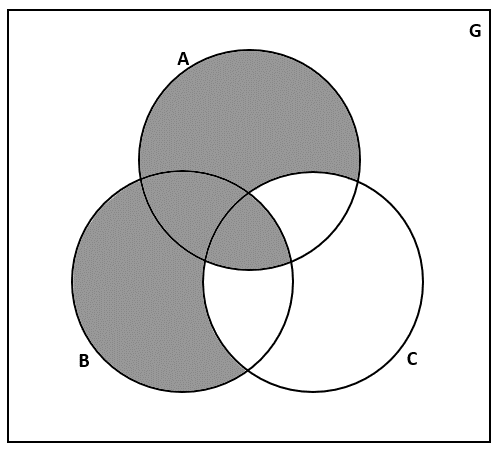
\includegraphics[width=5cm]{a).png}
\end{minipage}
\hfill
\begin{minipage}[t]{0.45\linewidth}
	\centering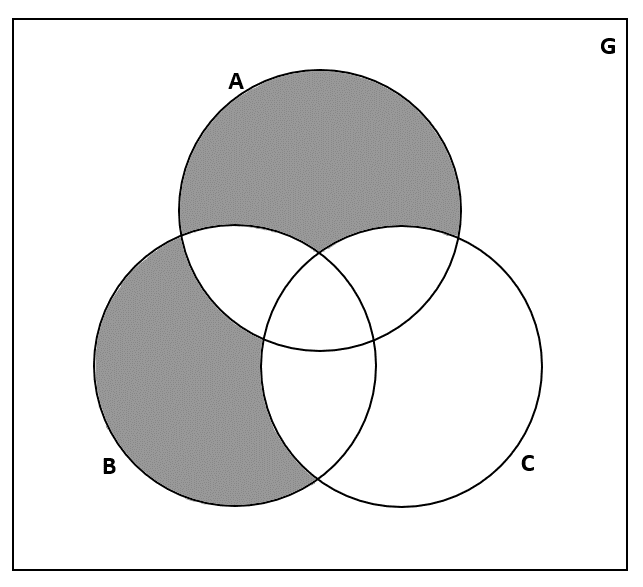
\includegraphics[width=5cm]{c).png}
\end{minipage}
\begin{parts}
	\part[2] Schreibe die grau markierte Mengen als Mengenterm.
\end{parts}
\begin{minipage}{0.45\linewidth}
	\centering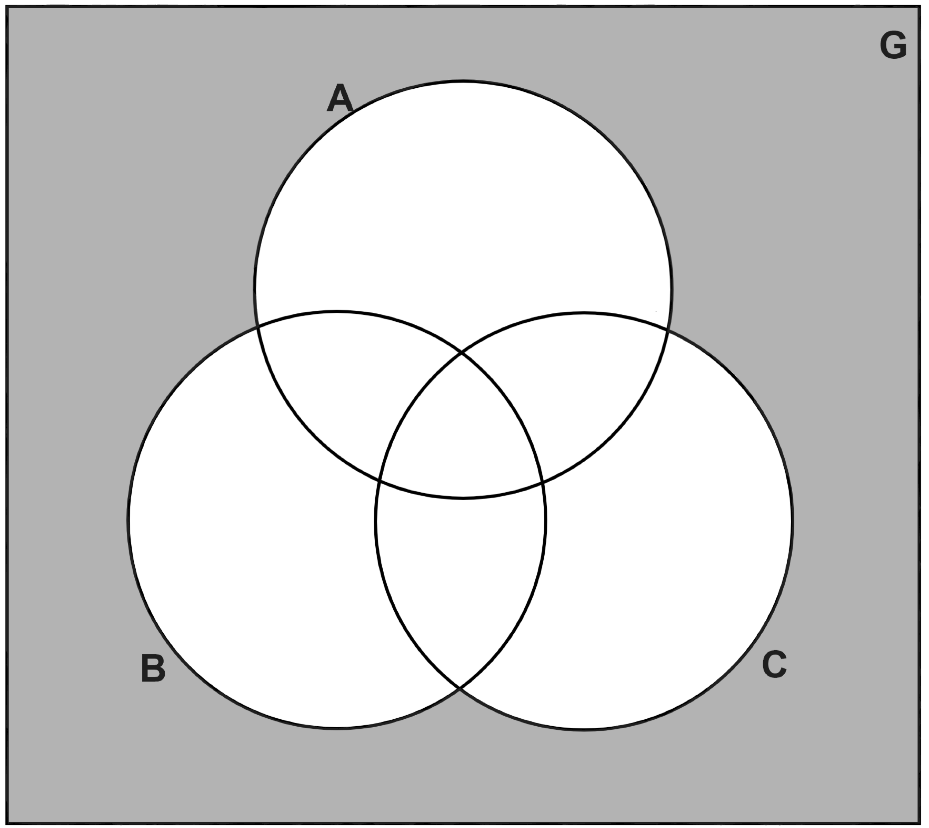
\includegraphics[width=5cm]{f).png}
\end{minipage}
\hfill
\begin{minipage}{0.45\linewidth}
	\centering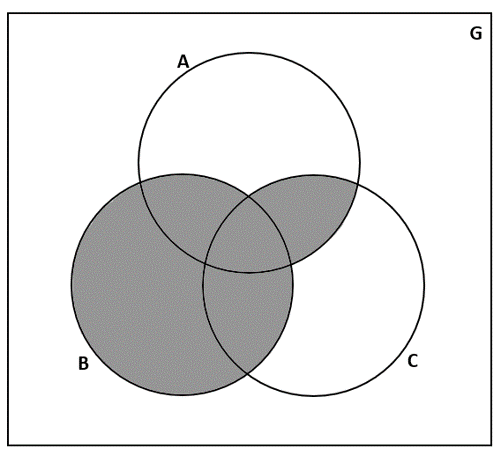
\includegraphics[width=5cm]{b).png}
\end{minipage}
\begin{parts}
	\part[2] Schreibe die grau markierte Mengen als Mengenterm.
\end{parts}
\begin{minipage}{0.45\linewidth}
	\centering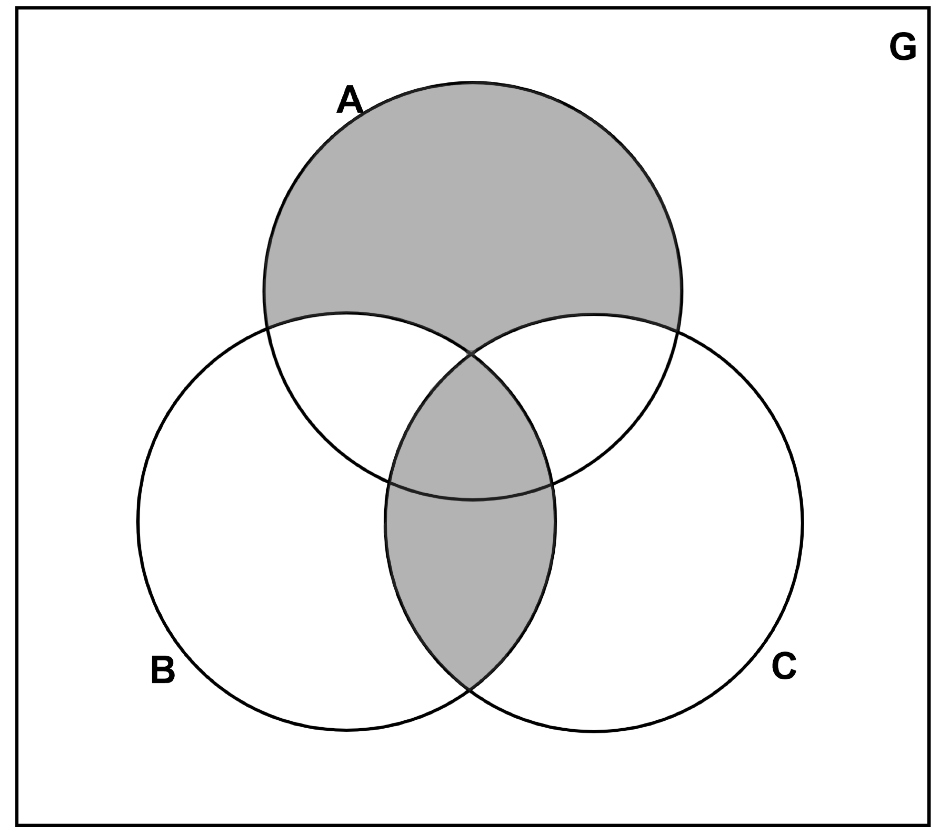
\includegraphics[width=5cm]{d).png}
\end{minipage}
\hfill
\begin{minipage}{0.45\linewidth}
	\centering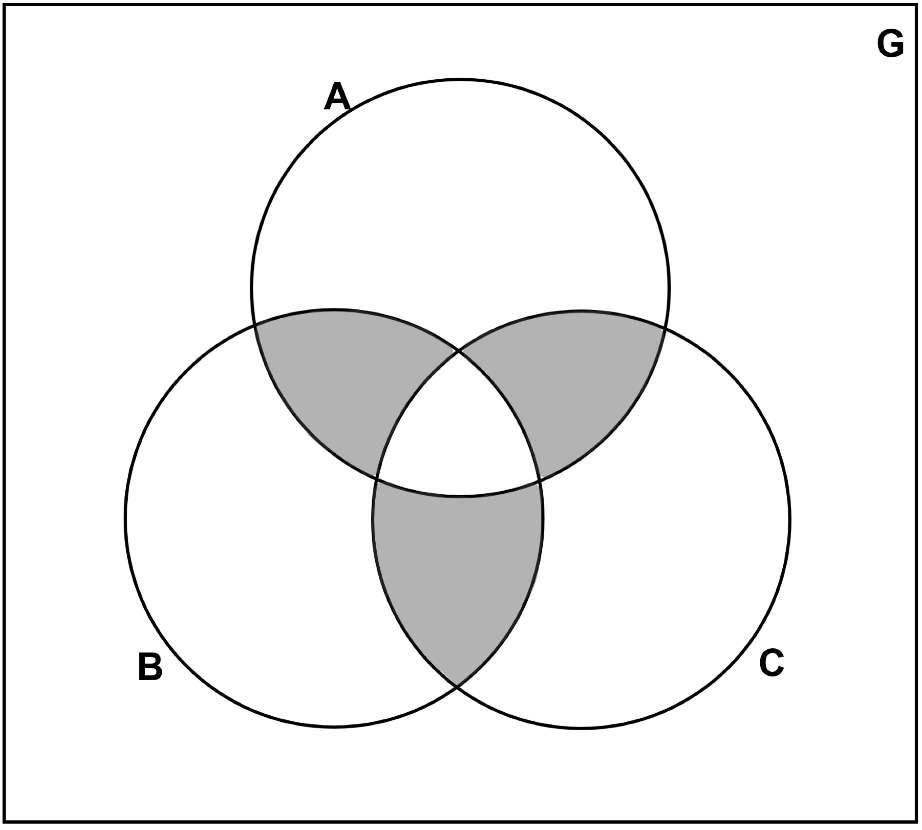
\includegraphics[width=5cm]{e).png}
\end{minipage}


%-------------------------------------------------------
\noaddpoints
\question[\totalpoints]
\addpoints
\begin{parts}
	\part[2] Schreibe die grau markierte Mengen als Mengenterm.
\end{parts}
\begin{minipage}{0.475\linewidth}
	\centering
	\begin{tikzpicture}[line cap=round,line join=round,>=triangle 45,x=1cm,y=1cm,scale=0.9]
		% Komplement von B
		\fill[gray!40] (-3,-3) rectangle (3,3);
		\fill[white] (-0.8,-0.8) circle (1.5);

		% Schnittmenge A und C
		\begin{scope}
			\clip (0,0.8) circle (1.5);
			\fill[gray!40] (0.8,-0.8) circle (1.5);
		\end{scope}

		\draw[color=black] (-3,-3) rectangle (3,3);
		\draw[color=black] (2.8,2.75) node {\footnotesize $G$};
		\draw[color=black] (0,0.8) circle (1.5);
		\draw[color=black] (-1,2.15) node {\footnotesize $A$};
		\draw[color=black] (0.8,-0.8) circle (1.5);
		\draw[color=black] (2,-2) node {\footnotesize $C$};
		\draw[color=black] (-0.8,-0.8) circle (1.5);
		\draw[color=black] (-2,-2) node {\footnotesize $B$};
	\end{tikzpicture}
\end{minipage}
\hfill
\begin{minipage}{0.5\linewidth}
	\centering
	\begin{tikzpicture}[line cap=round,line join=round,>=triangle 45,x=1cm,y=1cm,scale=0.9]
		% A vereinigt C
		\fill[gray!40] (0,0.8) circle (1.5);
		\fill[gray!40] (0.8,-0.8) circle (1.5);

		% Schnittmenge A und B wieder entfernen
		\begin{scope}
			\clip (0,0.8) circle (1.5);
			\clip (-0.8,-0.8) circle (1.5);
			\fill[white] (-3,-3) rectangle (3,3);
		\end{scope}

		\draw[color=black] (-3,-3) rectangle (3,3);
		\draw[color=black] (2.8,2.75) node {\footnotesize $G$};
		\draw[color=black] (0,0.8) circle (1.5);
		\draw[color=black] (-1,2.15) node {\footnotesize $A$};
		\draw[color=black] (0.8,-0.8) circle (1.5);
		\draw[color=black] (2,-2) node {\footnotesize $C$};
		\draw[color=black] (-0.8,-0.8) circle (1.5);
		\draw[color=black] (-2,-2) node {\footnotesize $B$};
	\end{tikzpicture}
\end{minipage}



%-------------------------------------------------------
\noaddpoints
\question[\totalpoints]
\addpoints
\begin{parts}
	\setcounter{partno}{1}
	\part[2] Schraffiere die folgenden Mengen im Venn Diagramm.
\end{parts}
\begin{minipage}[t]{0.45\linewidth}
	$(A\cup B)\cap (G\setminus (A\cup B))$
	\centering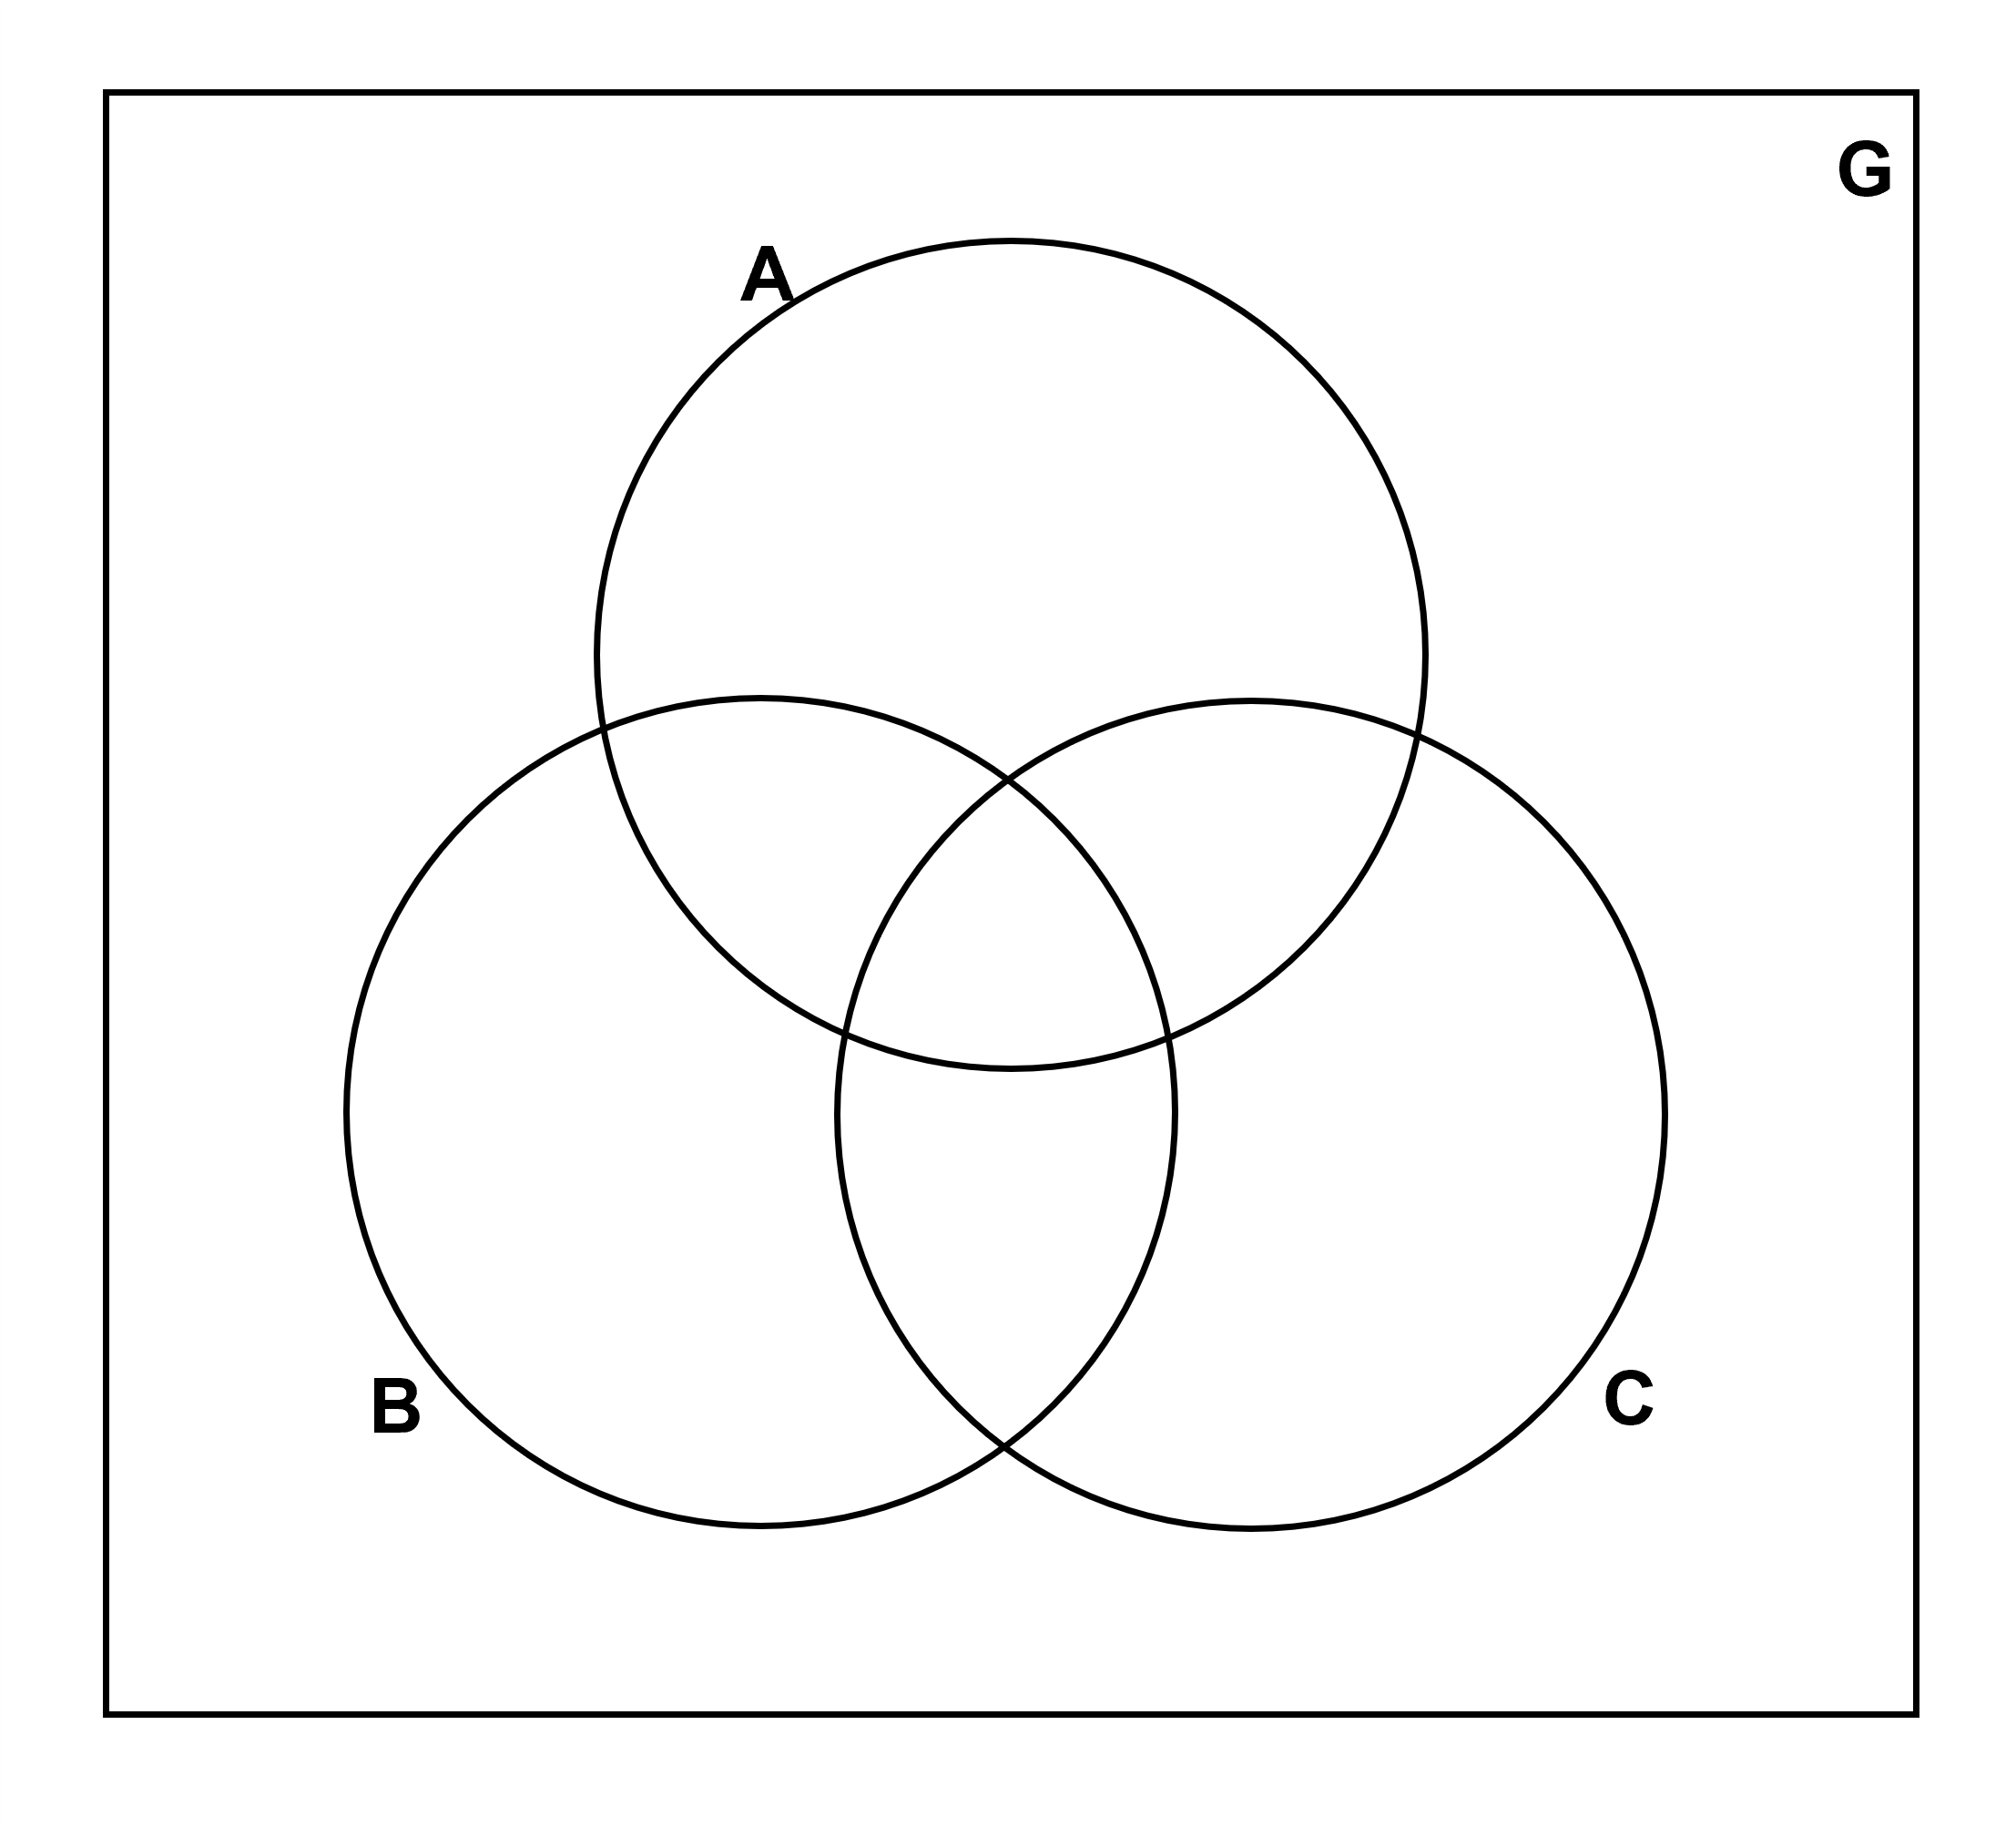
\includegraphics[width=5cm]{VennDiagramm.png}
\end{minipage}
\hfill
\begin{minipage}[t]{0.45\linewidth}
	$(A\setminus C)\cup(B\cap C)$
	\centering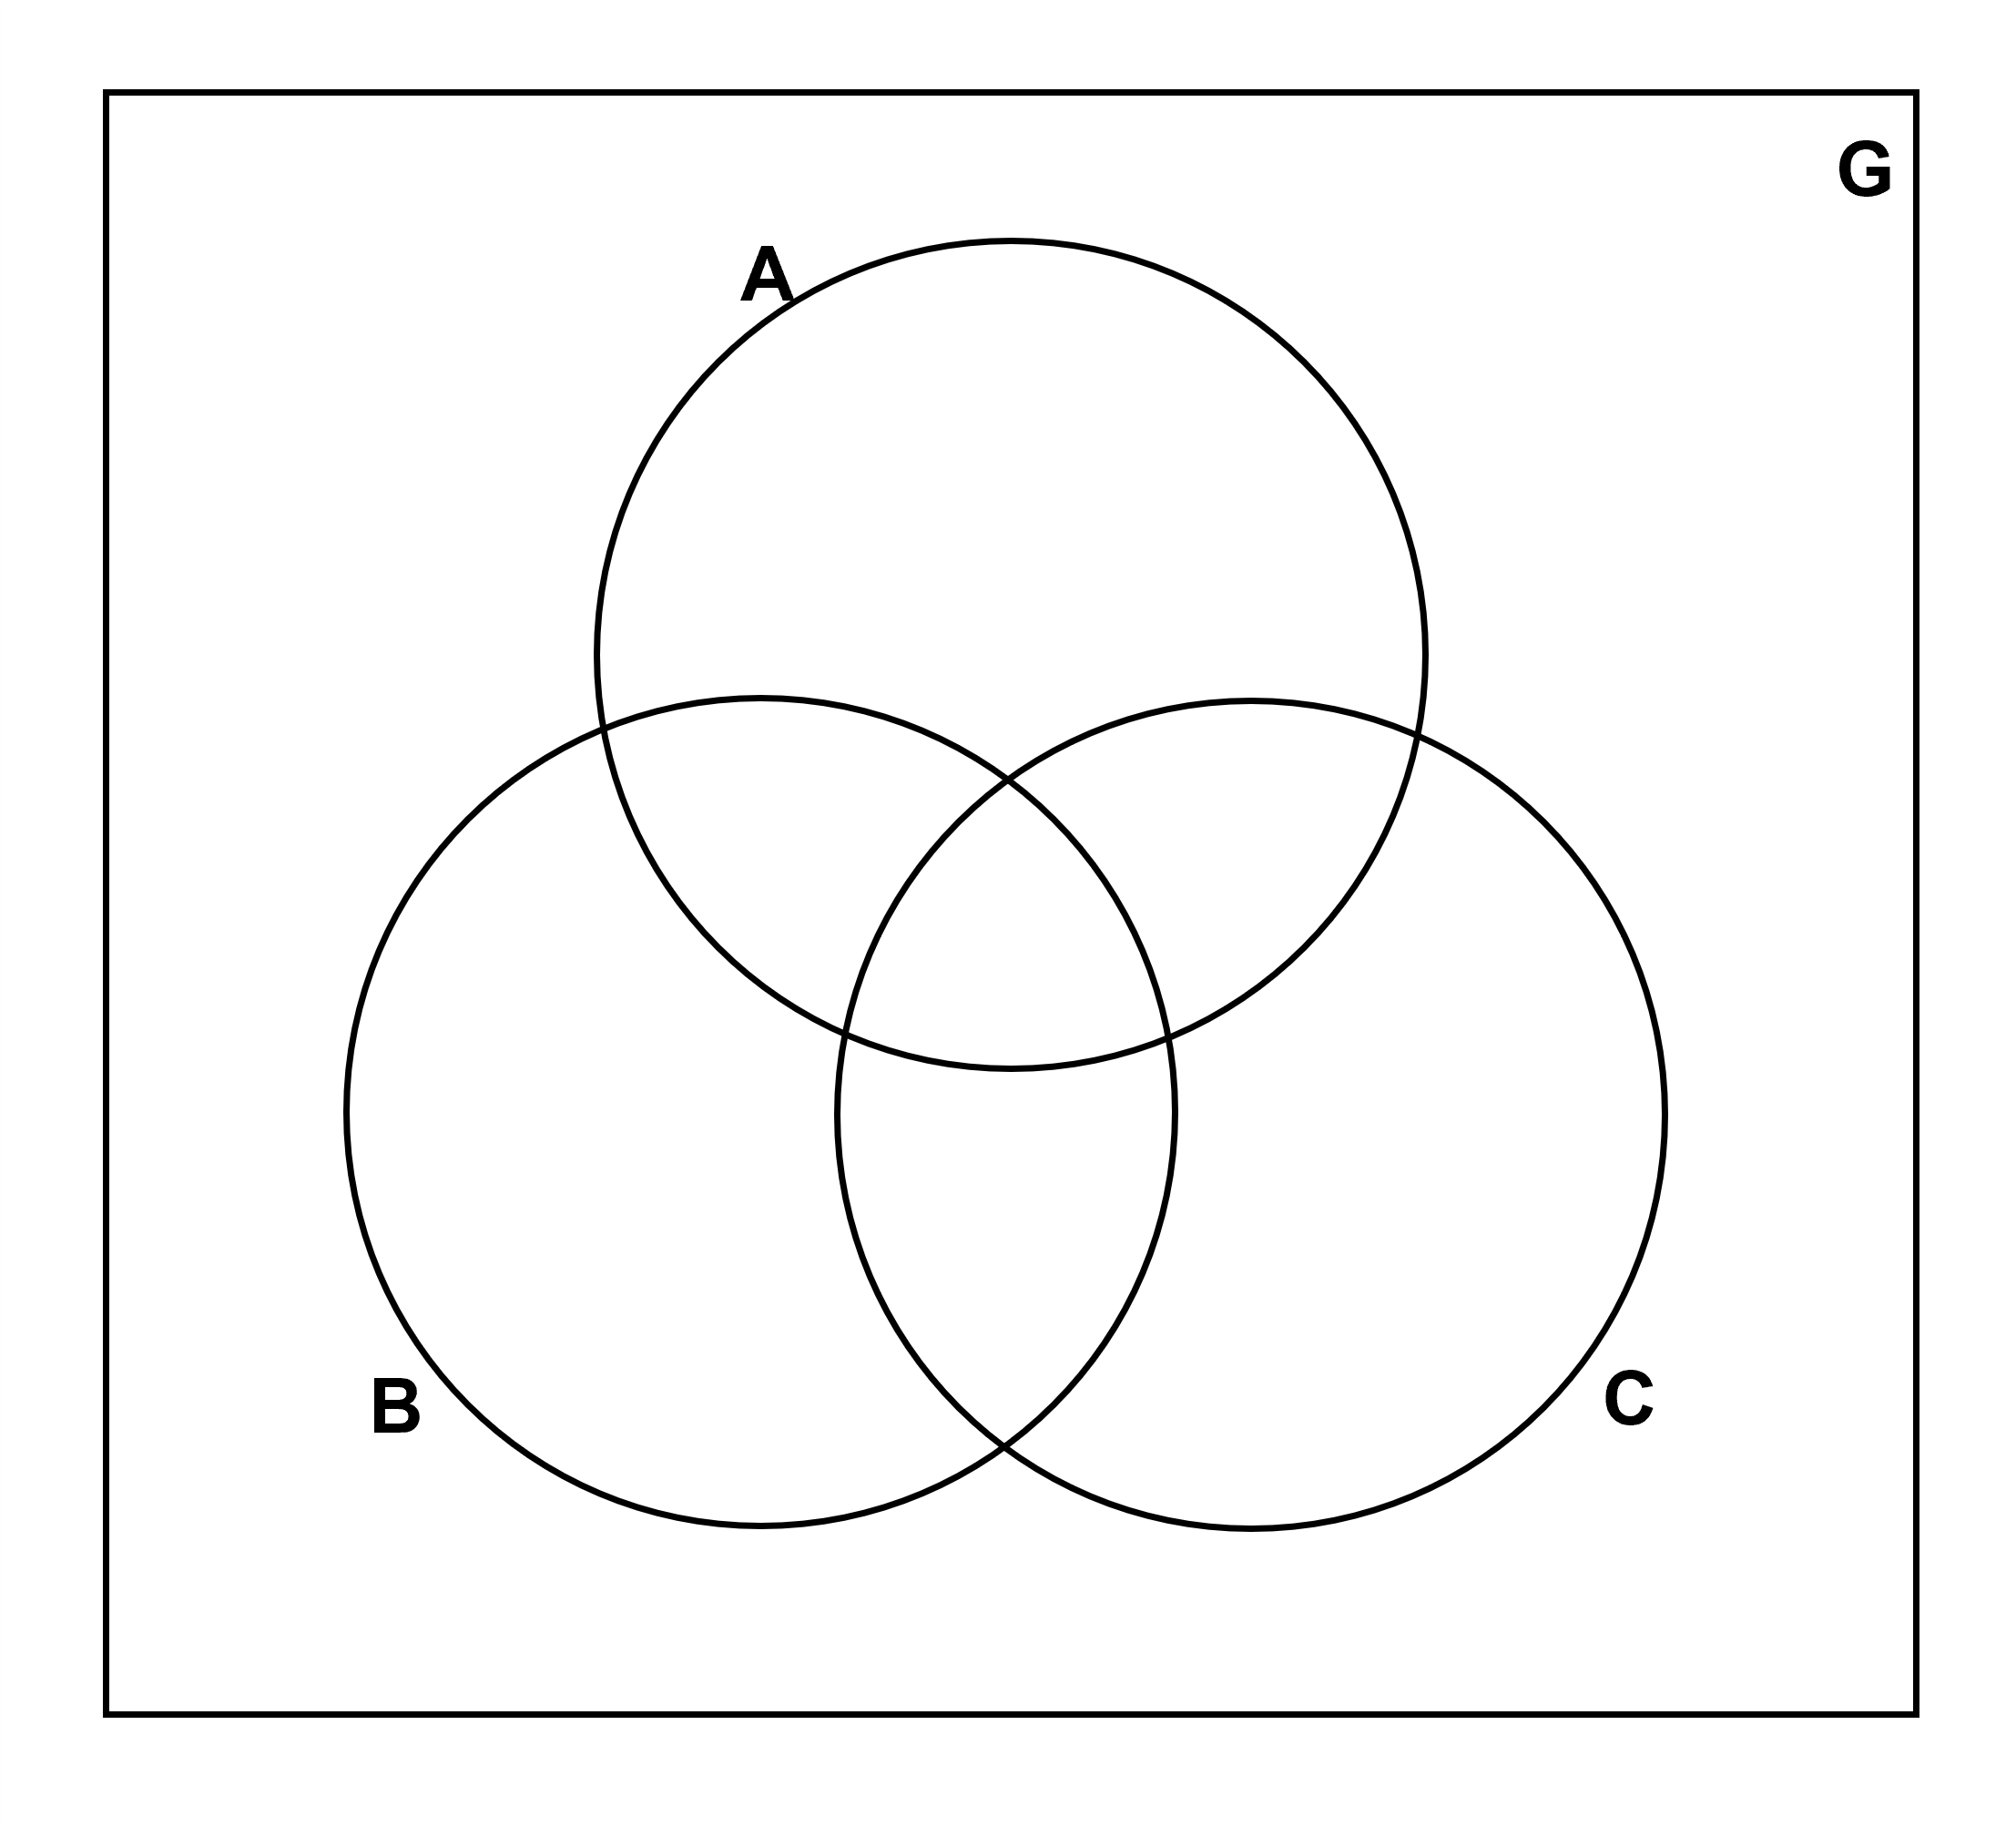
\includegraphics[width=5cm]{VennDiagramm.png}
\end{minipage}
\begin{parts}
	\setcounter{partno}{1}
	\part[2] Schraffiere die folgenden Mengen im Kreis-Diagramm.
\end{parts}
\begin{minipage}[t]{0.45\linewidth}
	$(A\cap B)\setminus (C\cap B)$
	\centering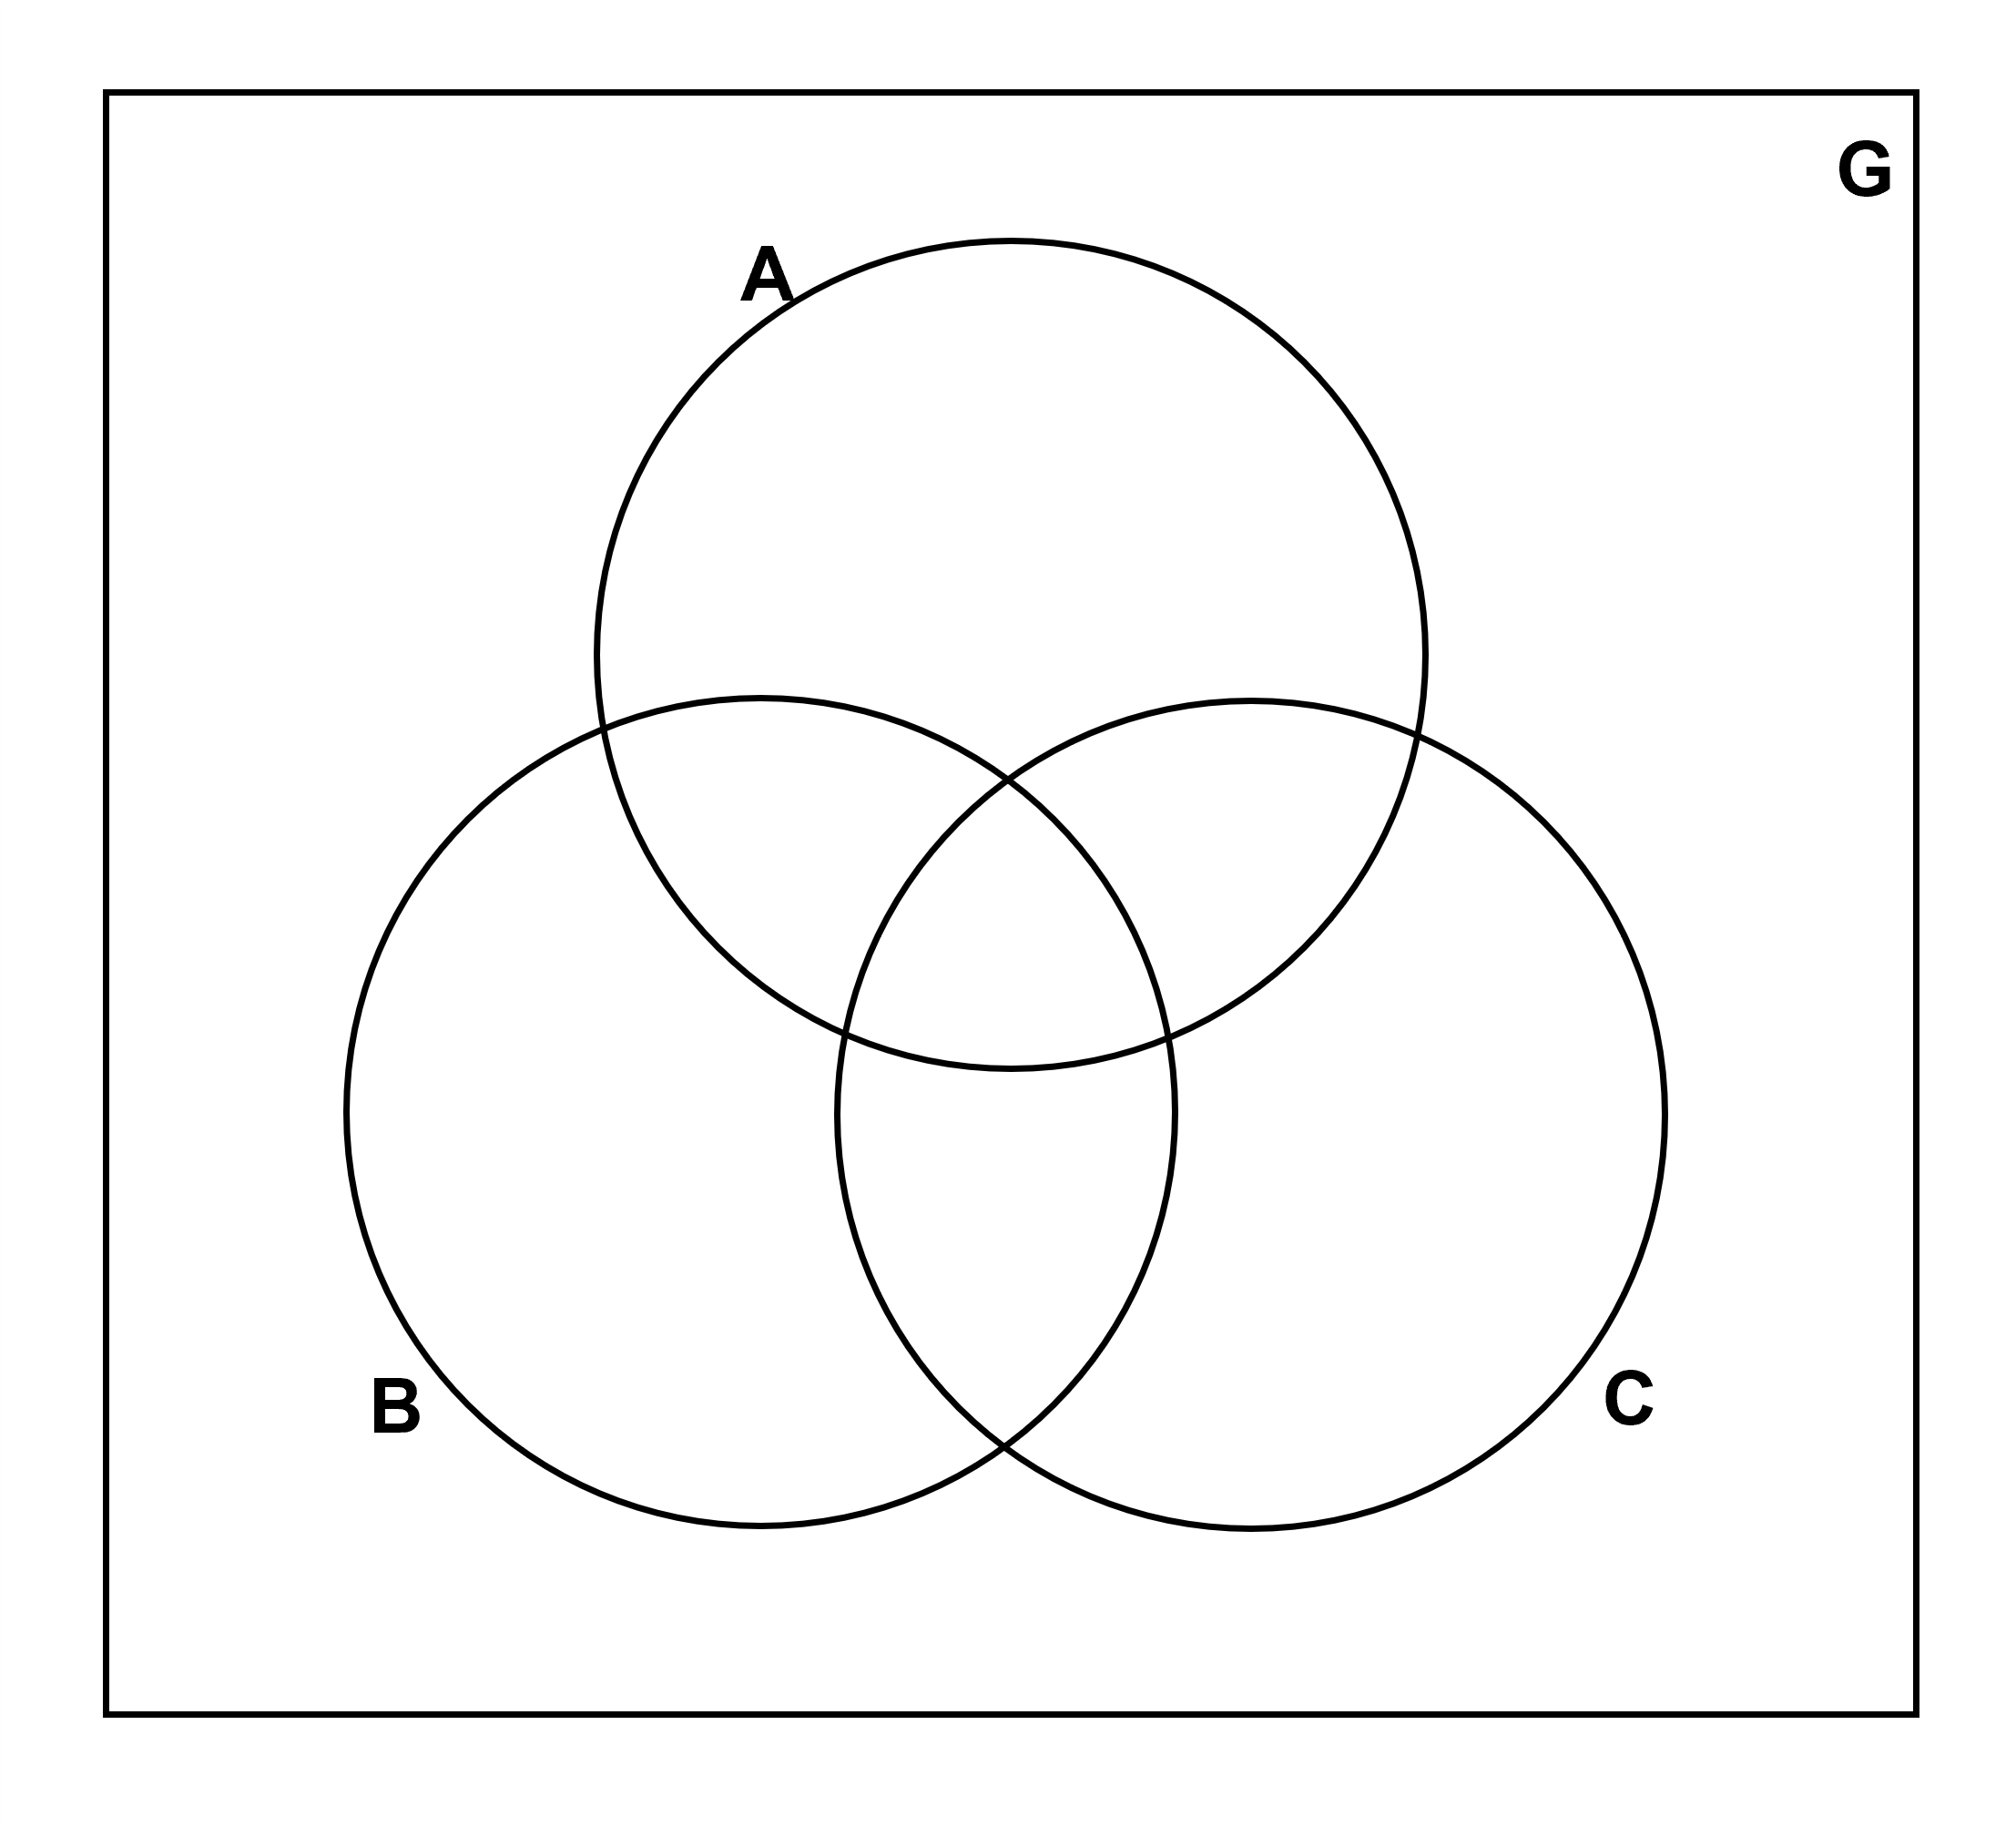
\includegraphics[width=5cm]{VennDiagramm.png}
\end{minipage}
\hfill
\begin{minipage}[t]{0.45\linewidth}
	$(C\cap B)\cup(A\cap(B\cap C))$
	\centering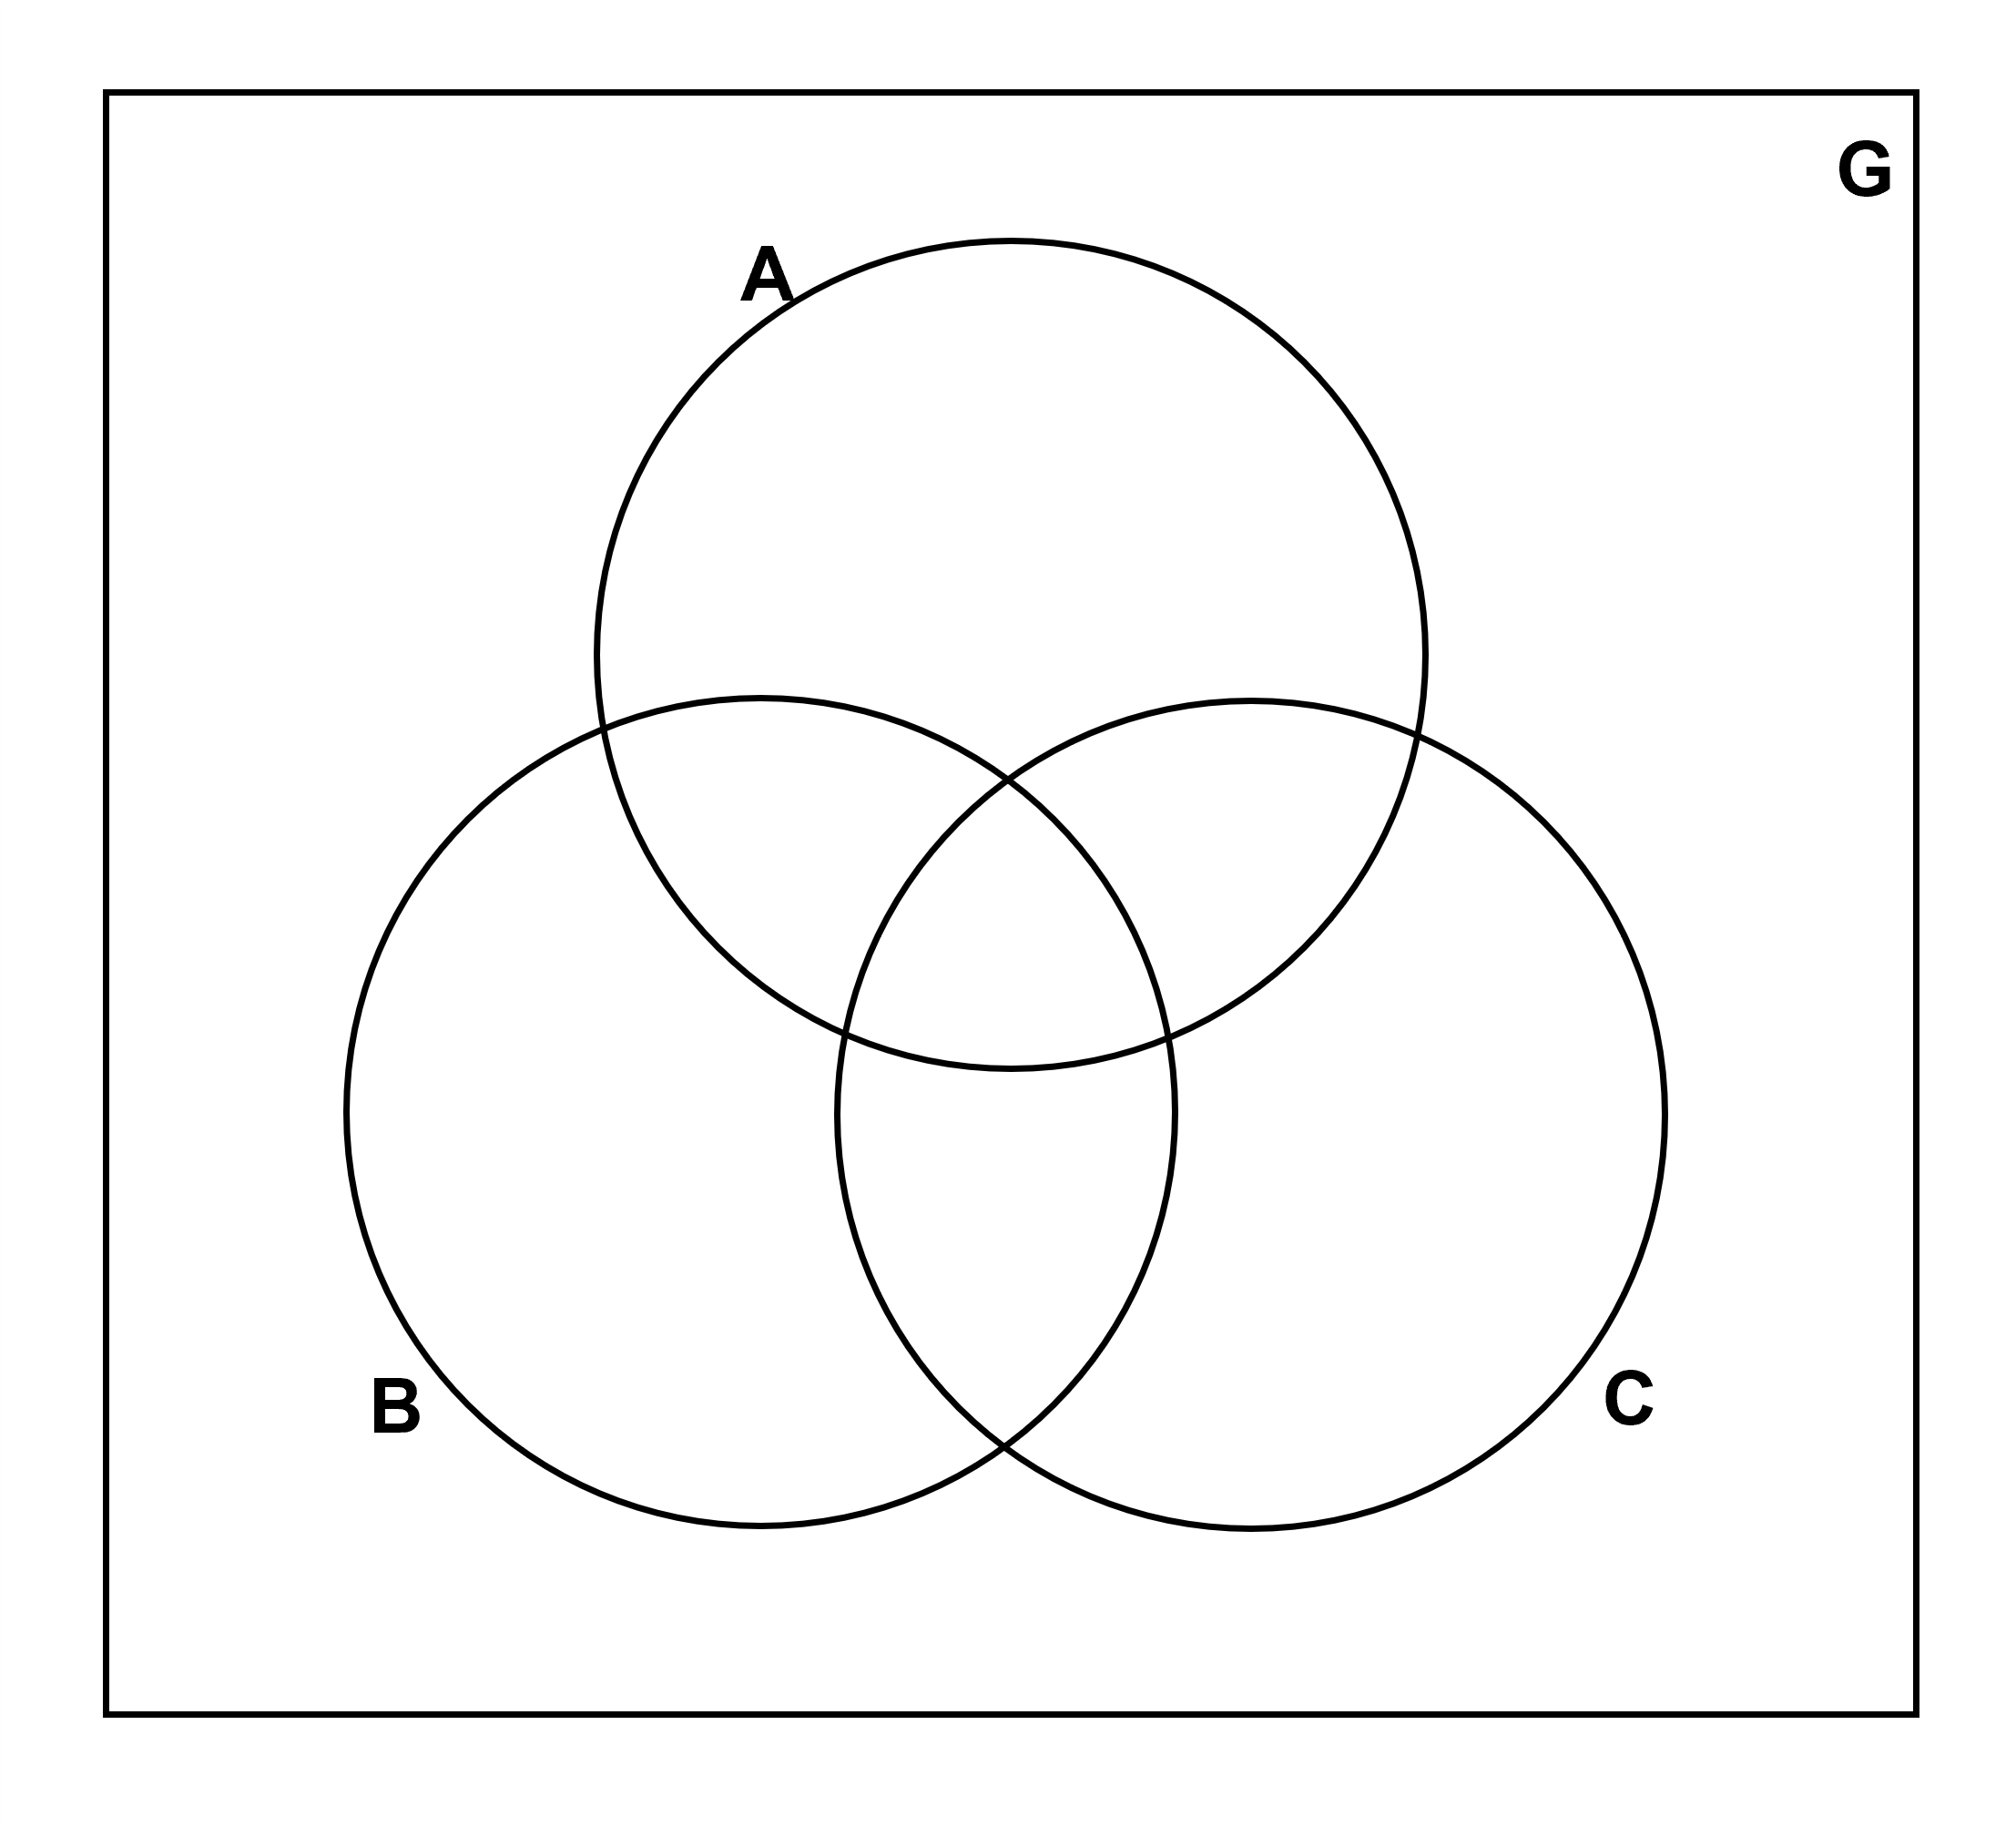
\includegraphics[width=5cm]{VennDiagramm.png}
\end{minipage}
\begin{parts}
	\setcounter{partno}{1}
	\part[2] Schraffiere die folgenden Mengen im Kreis-Diagramm.
\end{parts}
\begin{minipage}[t]{0.45\linewidth}
	$(A\cup B)\setminus (A\cap C)$
	\centering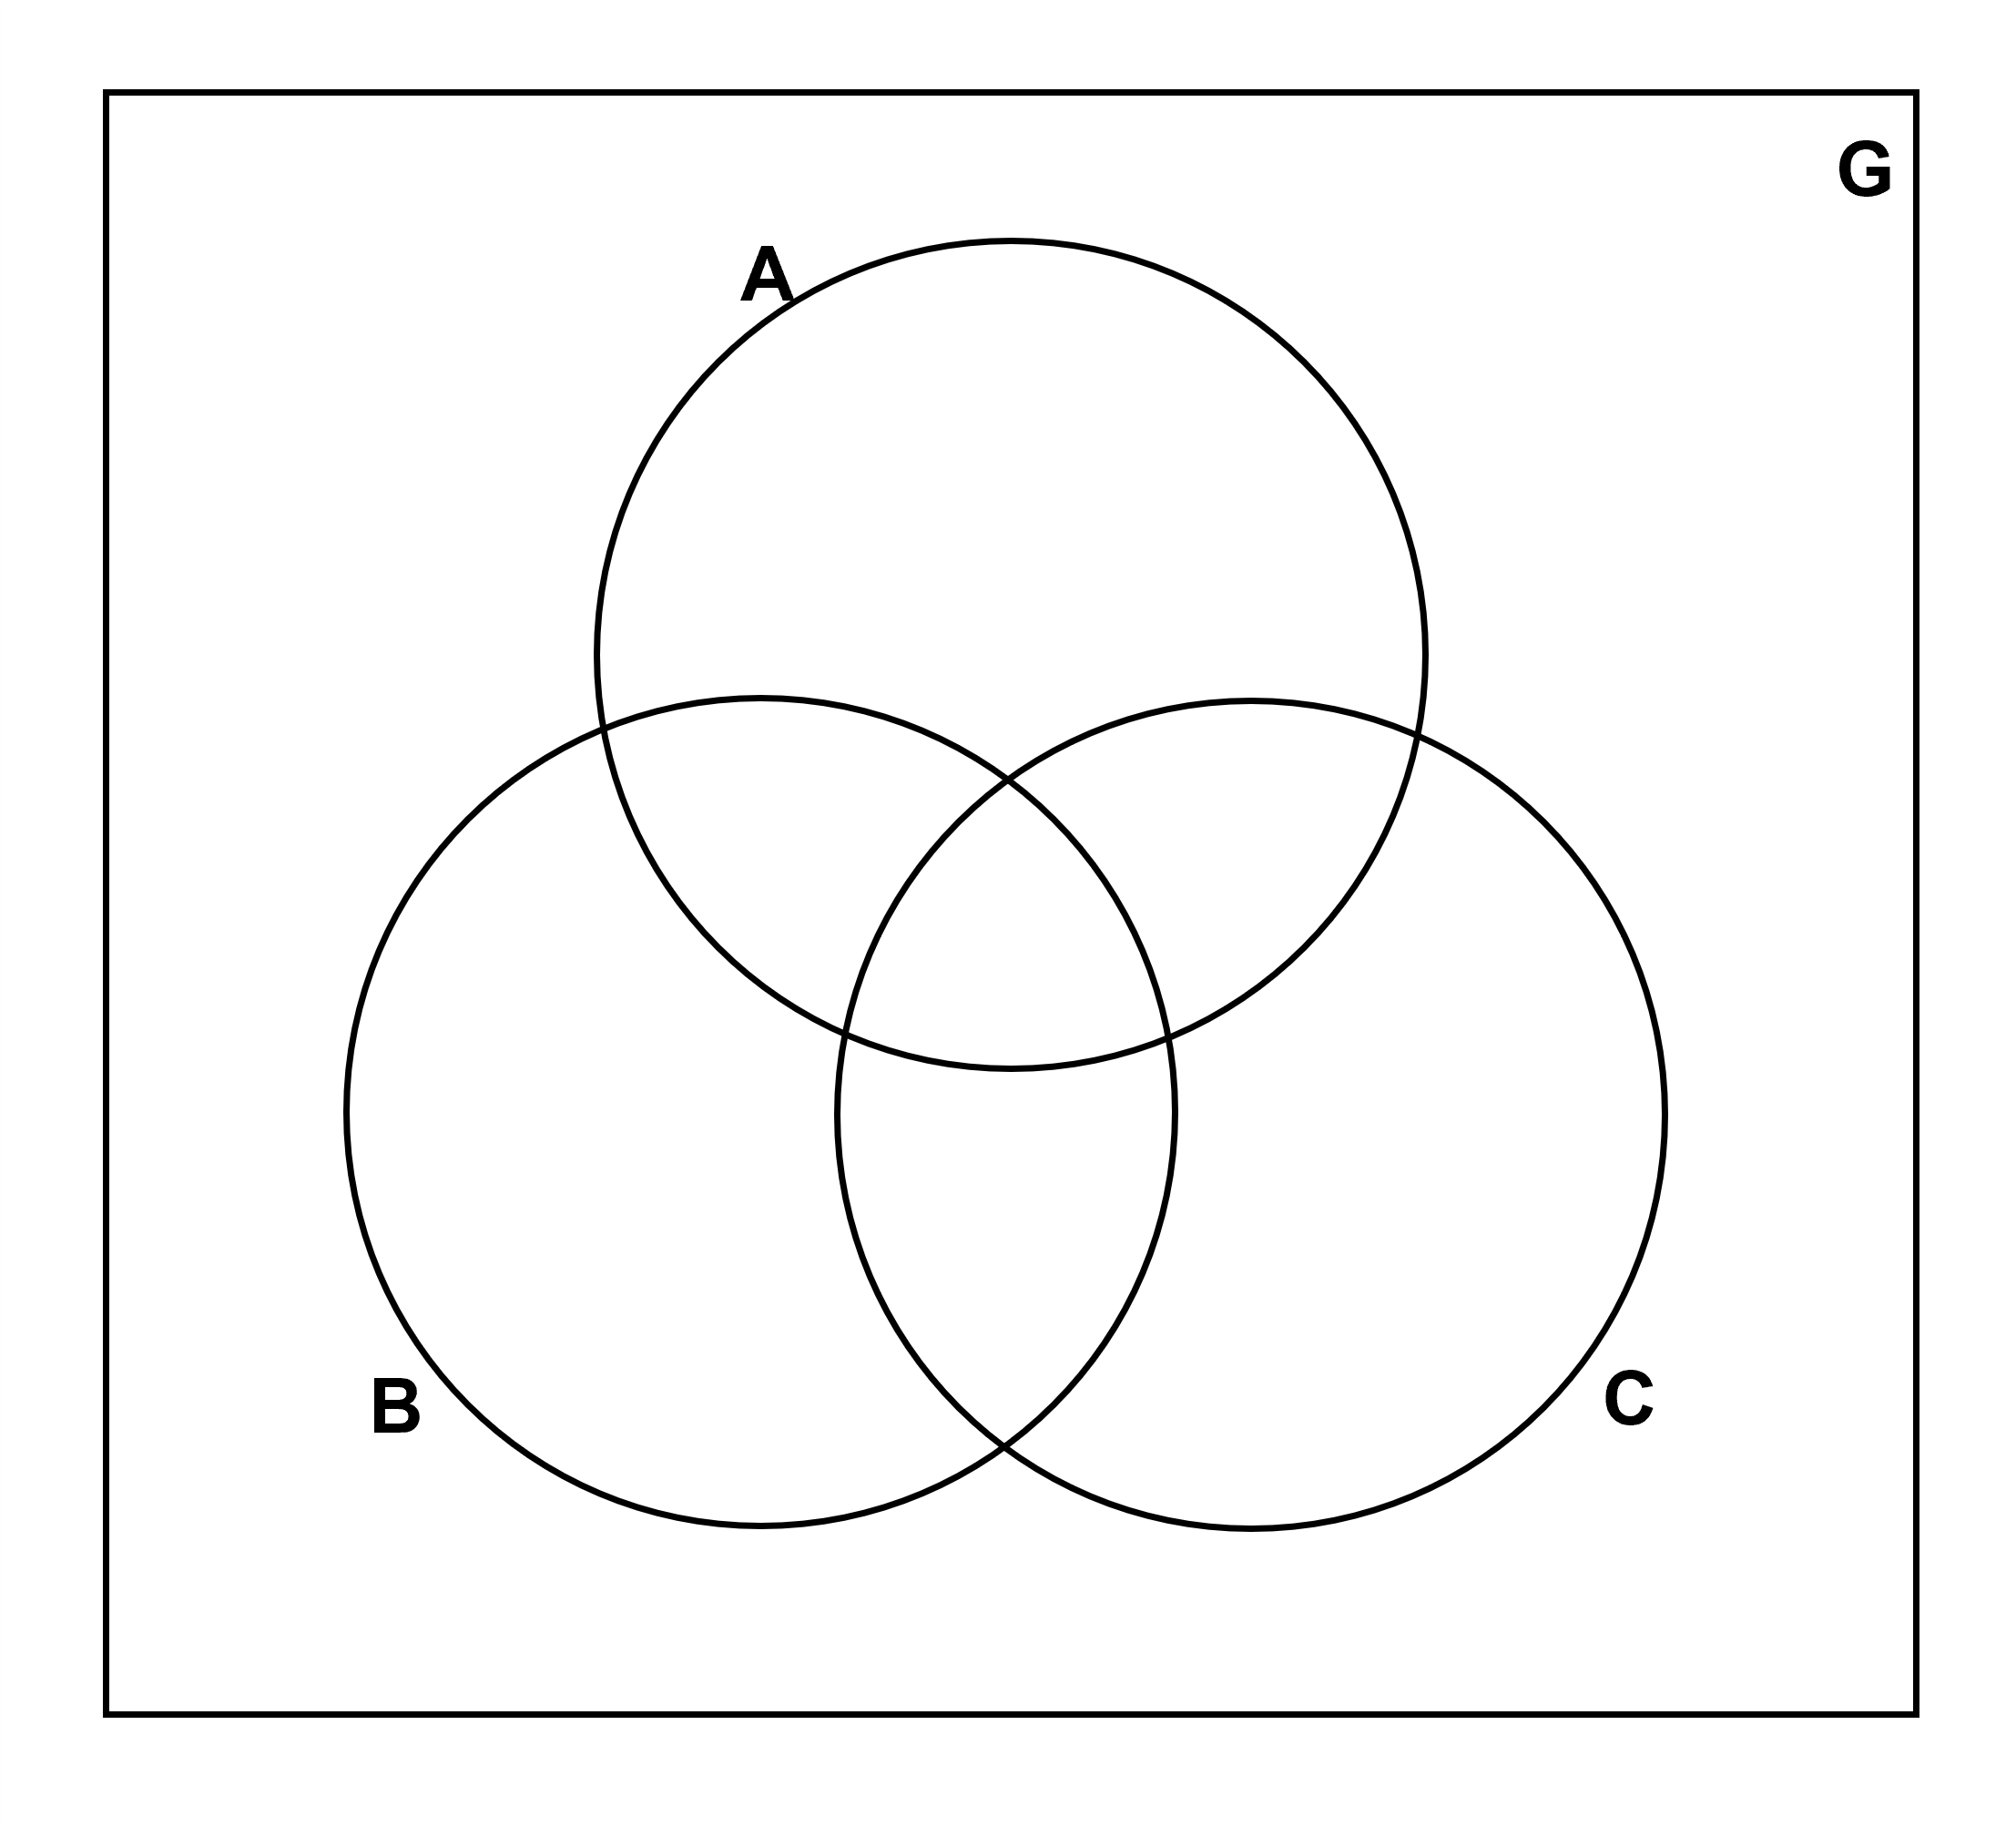
\includegraphics[width=5cm]{VennDiagramm.png}
\end{minipage}
\hfill
\begin{minipage}[t]{0.5\linewidth}
	$\left(C\setminus(A\cap B\cap C)\right)\cup\left(G\setminus(A\cup B\cup C)\right)$
	\centering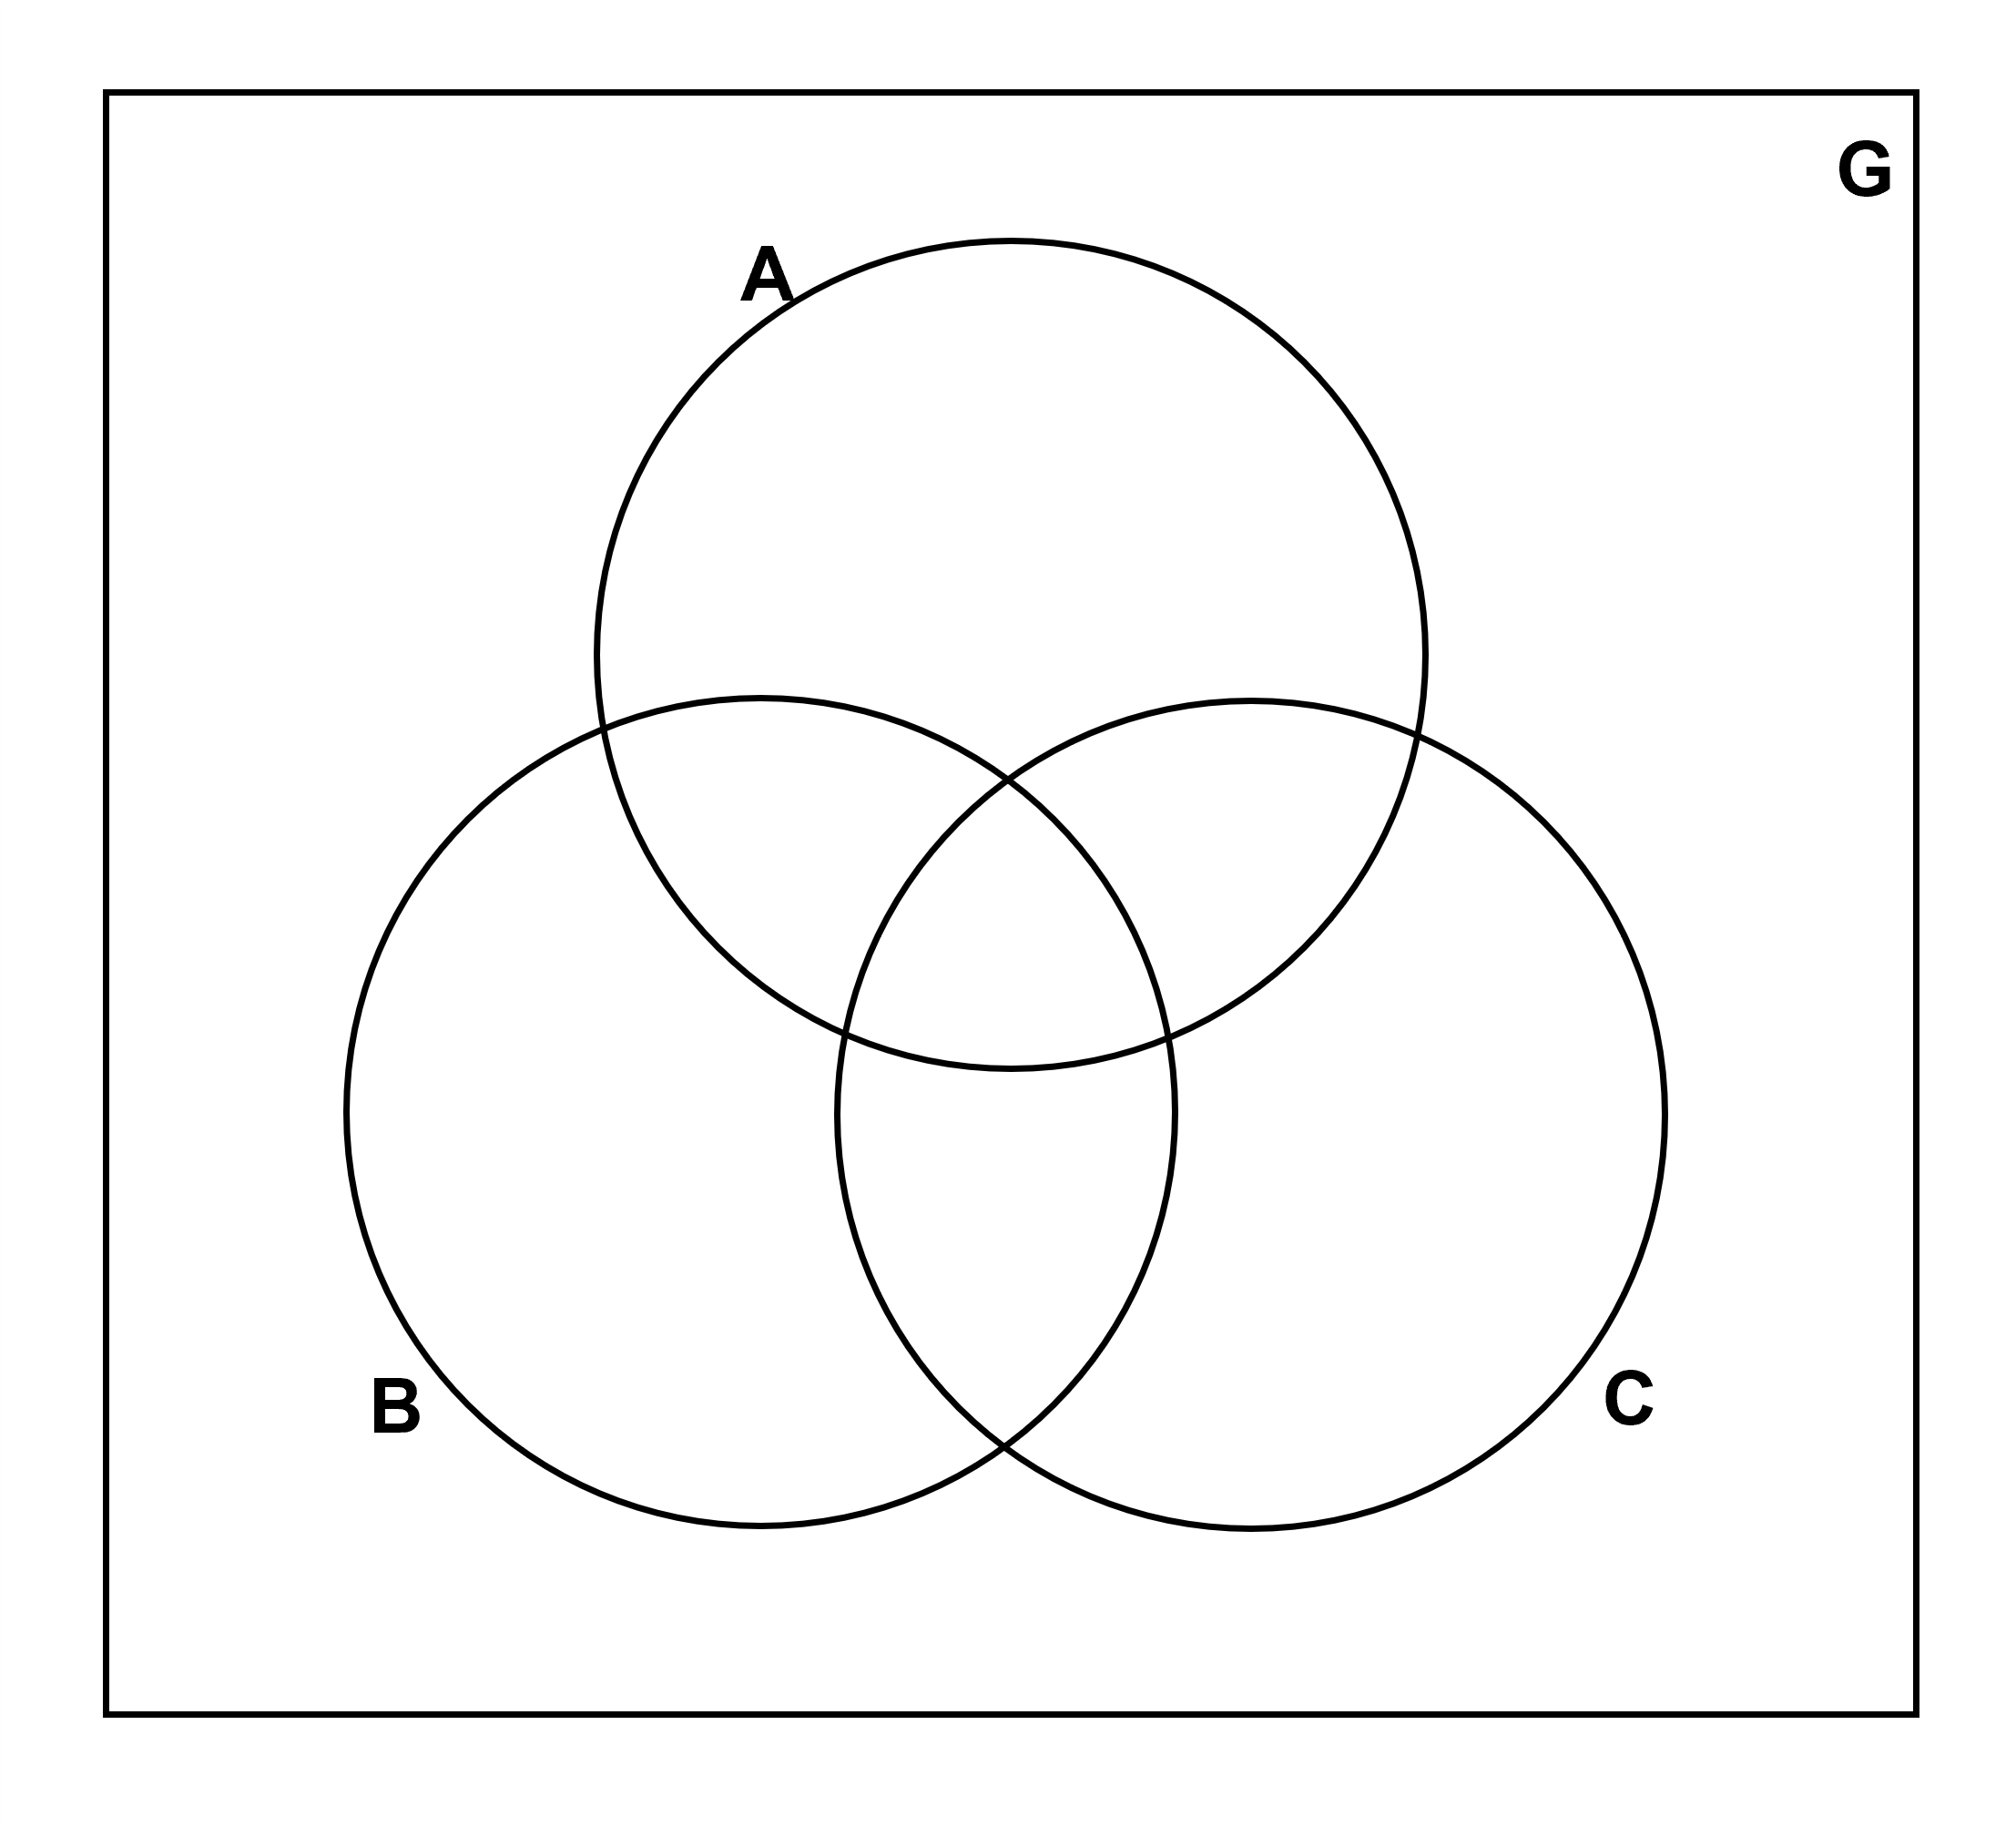
\includegraphics[width=5cm]{VennDiagramm.png}
\end{minipage}



%-------------------------------------------------------
\noaddpoints
\question[\totalpoints]
\addpoints
\begin{parts}
	\setcounter{partno}{1}
	\part[2] Schraffiere die folgenden Mengen im Venn Diagramm.
\end{parts}
\begin{minipage}[t]{0.475\linewidth}
	$(A\cup C)\cap B$
	\centering
	\begin{tikzpicture}[line cap=round,line join=round,>=triangle 45,x=1cm,y=1cm,scale=0.9]
		\draw[color=black] (-3,-3) -- (-3,3) -- (3,3) -- (3,-3) -- (-3,-3);
		\draw[color=black] (2.8,2.75) node {\footnotesize $G$};
		\draw[color=black] (0,0.8) circle (1.5);
		\draw[color=black] (-1,2.15) node {\footnotesize $A$};
		\draw[color=black] (0.8,-0.8) circle (1.5);
		\draw[color=black] (2,-2) node {\footnotesize $C$};
		\draw[color=black] (-0.8,-0.8) circle (1.5);
		\draw[color=black] (-2,-2) node {\footnotesize $B$};
	\end{tikzpicture}
\end{minipage}
\hfill
\begin{minipage}[t]{0.5\linewidth}
	$G\setminus (A\cup B)\cup(A\cap C)$
	\centering
	\begin{tikzpicture}[line cap=round,line join=round,>=triangle 45,x=1cm,y=1cm,scale=0.9]
		\draw[color=black] (-3,-3) -- (-3,3) -- (3,3) -- (3,-3) -- (-3,-3);
		\draw[color=black] (2.8,2.75) node {\footnotesize $G$};
		\draw[color=black] (0,0.8) circle (1.5);
		\draw[color=black] (-1,2.15) node {\footnotesize $A$};
		\draw[color=black] (0.8,-0.8) circle (1.5);
		\draw[color=black] (2,-2) node {\footnotesize $C$};
		\draw[color=black] (-0.8,-0.8) circle (1.5);
		\draw[color=black] (-2,-2) node {\footnotesize $B$};
	\end{tikzpicture}
\end{minipage}


%---------------------------------------------------------
\question[4]
Gegeben sind die folgenden Mengen $A=\left\{2,3,5,7,9,12,15\right\}$, $B=\left\{0,2,4,6,8,10,12\right\}$ und $C=\left\{0,-0.3,-1,\frac{-5}{2},-5\right\}$. Gib folgende Mengen an.
\begin{gridspace}{8.5}
   	\begin{enumerate}[label=(\alph*)]
   		\item $A\cap B=$
   		\item $B\cup \N=$
   		\item $C\cap \Z=$
   		\item $C\setminus \Q^-=$
   	\end{enumerate}
\end{gridspace}


%---------------------------------------------------------
\question[4]
Gegeben sind die folgenden Mengen $A=\left\{0,2,3,4,6,9,13,15\right\}$, $B=\left\{1,3,5,7,9,11,13\right\}$ und $C=\left\{0,3.2,3,\frac{5}{2},11\right\}$. Gib folgende Mengen an.
\begin{gridspace}{8.5}
   	\begin{enumerate}[label=(\alph*)]
   		\item $A\cup B=$
   		\item $A\cap \N=$
   		\item $C\cap \Z=$
   		\item $C\setminus \Q^+=$
   	\end{enumerate}
\end{gridspace}


%---------------------------------------------------------
\question[4]
Die folgenden Mengen $A=\left\{1,3,4,7,10,12,16\right\}$, $B=\left\{-2,3,-5,7,11,12,15\right\}$ und ${C=\left\{1,\frac{6}{5},4,5,7,12\right\}}$ sind gegeben. Schreibe die Mengen der untenstehenden Ausdrücke in aufzählender Form.
\begin{gridspace}{8.5}
	\begin{enumerate}[label=(\alph*)]
		\item $A\cup B=$
		\item $B\cap \N=$
		\item $C\cap \Z=$
		\item $C\setminus \Q^+=$
	\end{enumerate}
\end{gridspace}

%---------------------------------------------------------
\noaddpoints
\question[\totalpoints]
\addpoints
Verwandle $(a)$ und $(b)$ in einen Dezimalbruch und $(c)$ und $(d)$ in einen gewöhnlichen Bruch.
\begin{parcols}[2]
    \part[2] $\frac{2}{125}$ %0.012
	\part[2] $\frac{21}{16}$ %1.3125
	\part[2] $0.\overline{153}$ %17/111
	\part[2] $0.81\overline{6}$ %49/60
\end{parcols}


%---------------------------------------------------------
\noaddpoints
\question[\totalpoints]
\addpoints
Verwandle $(a)$ und $(b)$ in eine Dezimalzahl und $(c)$ und $(d)$ in einen gewöhnlichen Bruch.
\begin{parcols}[2]
    \part[2] $\frac{23}{16}$
    \part[2] $\frac{5}{22}$
    \part[2] $0.\overline{45}$
    \part[2] $0.6\overline{38}$
\end{parcols}


%---------------------------------------------------------
\noaddpoints
\question[\totalpoints]
\addpoints
Verwandle $(a)$ und $(b)$ in einen Dezimalbruch und $(c)$ und $(d)$ in einen gewöhnlichen Bruch.
\begin{parcols}[2]
	\part[2] $\frac{175}{4}$ %43.75
	\part[2] $\frac{29}{21}$ %1.380952...
	\part[2] $0.\overline{258}$ %86/333
	\part[2] $0.67\overline{5}$ %152/225
\end{parcols}


%---------------------------------------------------------
\noaddpoints
\question[\totalpoints]
\addpoints
Verwandle $(a)$ und $(b)$ in eine Dezimalzahl und $(c)$ und $(d)$ in einen gewöhnlichen Bruch.
\begin{parcols}[2]
    \part[2] $0.\overline{365}$
    \part[2] $9.1\overline{27}$
\end{parcols}


%---------------------------------------------------------
\noaddpoints
\question[\totalpoints]
\addpoints
\begin{parts}
	\part[4] Stelle zu jeder dieser Zahlen die Primfaktorzerlegung her.
	\begin{itemcols}[2]
		\item $6776$
		\item $2520$
	\end{itemcols}
	\part[4] Benutze die Primfaktorzerlegung, um das $\kgV$ und den $\ggT$ der zwei Zahlen $135$ und $294$ zu berechnen.
\end{parts}


%---------------------------------------------------------
\noaddpoints
\question[\totalpoints]
\addpoints
\begin{parts}
	\part[4] Stelle zu jeder dieser Zahlen die Primfaktorzerlegung her.
	\begin{itemcols}[2]
		\item $7128$
		\item $2772$
	\end{itemcols}
	\part[4] Benutze die Primfaktorzerlegung, um das $\kgV$ und den $\ggT$ der zwei Zahlen $168$ und $360$ zu berechnen.
\end{parts}

%---------------------------------------------------------
\noaddpoints
\question[\totalpoints] % ggT und kgV
\addpoints
Benutze die Primfaktorzerlegung, um die folgenden $\kgV$ und $\ggT$ zu berechnen.
\begin{parts}
    \part[3] Berechne das $\kgV(135,294)$.
    \part[3] Berechne den $\ggT(168,588)$
\end{parts}


%---------------------------------------------------------
\noaddpoints
\question[\totalpoints] % ggT und kgV
\addpoints
Benutze die Primfaktorzerlegung, um die folgenden $\kgV$ und $\ggT$ zu berechnen.
\begin{parts}
    \part[3] Berechne das $\kgV(252,120)$.
    \part[3] Berechne den $\ggT(315,150)$
\end{parts}

%---------------------------------------------------------
\question[2]
Entscheide in der Tabelle unten, ob die Aussagen wahr oder falsch sind. Die Antworten müssen nicht begründet werden.\newline
\begin{small}
    Bewertung: Für $0-2$ korrekte Antworten gibt es keine Punkte; $3$ korrekte Antworten einen Punkt und falls alle Antworten korrekt sind, gibt es $2$ Punkte.
\end{small}
\begingroup
\renewcommand{\arraystretch}{1.5}
\begin{table}[h]
    \centering
    \begin{tabular}{|p{12cm}|c|c|}\hline
         & wahr & falsch \\\hline
        Alle möglichen Dezimalzahlen gehören zu den rationalen Zahlen. & & \\\hline
        Eine Zahl ist durch $3$ teilbar, wenn ihre Quersumme ein Vielfaches von $3$ ist. & & \\\hline
        Es gibt eine natürliche Zahl, die zwei verschiedene Primfaktorzerlegungen besitzt.  & & \\\hline
        Es gibt keine natürliche Zahl, die zwei verschiedene Primfaktorzerlegungen besitzt.  & & \\\hline
        Jede natürliche Zahl grösser als 1 besitzt eine Primfaktorzerlegung. & & \\\hline
        Die Zahl $2645379$ ist durch $3$ teilbar. & & \\\hline
        Die Zahl $4815276$ ist durch $3$ teilbar. & & \\\hline
        In einem abgeschlossenen Intervall gehören die Grenzen nicht dazu. & & \\\hline
        In einem offenen Intervall gehören die Grenzen nicht dazu. & & \\\hline
        Eine unendliche Menge besitzt unendliche viele Teilmengen. & & \\\hline
        Die Gegenzahl einer Gegenzahl ist wieder die ursprüngliche Zahl. & & \\\hline
        Addiert man eine Zahl und ihre Gegenzahl, erhält man $0$. & & \\\hline
    \end{tabular}
\end{table}
\endgroup


%---------------------------------------------------------
\noaddpoints
\question[\totalpoints]
\addpoints
Zeichne die folgenden Mengen als Intervalle in die Zahlengerade ein.
\begin{parts}
	\part[2] $\left\{x\in \R\:|-4\leq x < 2\right\}=$
\end{parts}\vspace{1cm}
\begin{figure}[H]
    \centering
    \begin{tikzpicture}[line cap=round,line join=round,>=triangle 45,x=1cm,y=1cm]
        \draw[->](-5,0) --(8,0);
        \foreach \x in {-4.,-3.,-2.,-1.,0.,1.,2.,3.,4.,5.,6.,7.}
        \draw[shift={(\x,0)},color=black] (0pt,2pt) -- (0pt,-2pt) ;%node[below] {\footnotesize $\x$};
        \draw[color=black] (8,0) node[right] {$\R$};
    \end{tikzpicture}
\end{figure}\vspace{1cm}
\begin{parts}\setcounter{partno}{1}
	\part[2] $\R\setminus\left[1.5,2.5\right]=$
\end{parts}\vspace{1cm}
\begin{figure}[H]
    \centering
    \begin{tikzpicture}[line cap=round,line join=round,>=triangle 45,x=1.0cm,y=1cm]
        \draw[->](-5,0) --(8,0);
        \foreach \x in {-4.,-3.,-2.,-1.,0.,1.,2.,3.,4.,5.,6.,7.}
        \draw[shift={(\x,0)},color=black] (0pt,2pt) -- (0pt,-2pt) ;%node[below] {\footnotesize $\x$};
        \draw[color=black] (8,0) node[right] {$\R$};
    \end{tikzpicture}
\end{figure}


%---------------------------------------------------------
\noaddpoints
\question[\totalpoints]
\addpoints
Zeichne die folgenden Mengen als Intervalle in die Zahlengerade ein.
\begin{parts}
	\part[2] $\left\{x\in \R\:|-3\leq x < 4\right\}=$
\end{parts}\vspace{1cm}
\begin{figure}[H]
    \centering
    \begin{tikzpicture}[line cap=round,line join=round,>=triangle 45,x=1cm,y=1cm]
        \draw[->](-5,0) -- (8,0);
        \foreach \x in {-4.,-3.,-2.,-1.,0.,1.,2.,3.,4.,5.,6.,7.}
        \draw[shift={(\x,0)},color=black] (0pt,2pt) -- (0pt,-2pt) ;%node[below] {\footnotesize $\x$};
        \draw[color=black] (8,0) node[right] {$\R$};
    \end{tikzpicture}
\end{figure}\vspace{1cm}
\begin{parts}
	\setcounter{partno}{1}
	\part[2] $\R\setminus\left[-1,2\right]=$
\end{parts}\vspace{1cm}
\begin{figure}[H]
    \centering
    \begin{tikzpicture}[line cap=round,line join=round,>=triangle 45,x=1.0cm,y=1cm]
        \draw[->](-5,0) -- (8,0);
        \foreach \x in {-4.,-3.,-2.,-1.,0.,1.,2.,3.,4.,5.,6.,7.}
        \draw[shift={(\x,0)},color=black] (0pt,2pt) -- (0pt,-2pt) ;%node[below] {\footnotesize $\x$};
        \draw[color=black] (8,0) node[right] {$\R$};
    \end{tikzpicture}
\end{figure}


%---------------------------------------------------------
\noaddpoints
\question[\totalpoints]
\addpoints
Zeichne die folgenden Mengen als Intervalle in die Zahlengerade ein und gib die Teilmenge als Ausdruck von Intervallen an.
\begin{parts}
	\part[2] $\left\{x\in \R\:|-6< x \leq 3\right\}=$
\end{parts}\vspace{1cm}
\begin{figure}[H]
	\centering
	\begin{tikzpicture}[line cap=round,line join=round,>=triangle 45,x=1cm,y=1cm]
		\draw[->](-5,0) --(8,0);
		\foreach \x in {-4.,-3.,-2.,-1.,0.,1.,2.,3.,4.,5.,6.,7.}
		\draw[shift={(\x,0)},color=black] (0pt,2pt) -- (0pt,-2pt) ;%node[below] {\footnotesize $\x$};
		\draw[color=black] (8,0) node[right] {$\R$};
	\end{tikzpicture}
\end{figure}\vspace{1cm}
\begin{parts}\setcounter{partno}{1}
	\part[2] $\R\setminus\left]-4.25,1.775\right[=$
\end{parts}\vspace{1cm}
\begin{figure}[H]
	\centering
	\begin{tikzpicture}[line cap=round,line join=round,>=triangle 45,x=1.0cm,y=1cm]
		\draw[->](-5,0) --(8,0);
		\foreach \x in {-4.,-3.,-2.,-1.,0.,1.,2.,3.,4.,5.,6.,7.}
		\draw[shift={(\x,0)},color=black] (0pt,2pt) -- (0pt,-2pt) ;%node[below] {\footnotesize $\x$};
		\draw[color=black] (8,0) node[right] {$\R$};
	\end{tikzpicture}
\end{figure}


%---------------------------------------------------------
\newpage
\noaddpoints
\question[\totalpoints]
\addpoints
Stelle folgende Teilmengen von $\R$ als Intervalle dar.
\begin{parts}
	\part[2] $\left\{x\in \R\:|-4\leq x < 2 \text{ oder } 2 < x \leq 3.4 \right\}=$
    \part[2] $\R\setminus\left[1.5,2.5\right]=$
\end{parts}

%---------------------------------------------------------
\noaddpoints
\question[\totalpoints]
\addpoints
Stelle folgende Teilmengen von $\R$ als Intervalle dar.
\begin{parts}
	\part[2] $\left\{x\in \R\:| x\leq-3 \text{ oder } x\geq 3\right\}=$
	\part[2] $\R_0^+\setminus\left\{1.3,5\right\}=$
\end{parts}

%---------------------------------------------------------
\noaddpoints
\question[\totalpoints]
\addpoints
Stelle die folgenden Teilmengen von $\R$ als Intervalle dar.
\begin{parts}
	\part[2] $\left\{x\in \R\:| x\leq-3.2\right\}=$
	\part[2] $\R_0^+\setminus\left\{1.3,5\right\}=$
\end{parts}

%---------------------------------------------------------
\noaddpoints
\question[\totalpoints]
\addpoints
Stelle die folgenden Teilmengen von $\R$ als Intervalle dar.
\begin{parts}
	\part[2] $\left\{x\in \R\:\vert -3.2 < x < 17.7\right\}=$
	\part[2] $\R_0^+\setminus\left\{1.3\right\}=$
\end{parts}

%---------------------------------------------------------
\noaddpoints
\question[\totalpoints]
\addpoints
Stelle die folgenden Teilmengen von $\R$ als Intervalle dar.
\begin{parts}
	\part[2] $\left\{x\in \R\:| x\geq-3.2\right\}=$
	\part[2] $\R_0^-\setminus\left[-6,-2\right]=$
\end{parts}


%---------------------------------------------------------
\noaddpoints
\question[\totalpoints]
\addpoints
Berechne den Wert der folgenden Terme, indem du alle Betragsstriche auflöst.
\begin{parts}
	\part[2] $\abs{-5-\abs{2-3}}+2=$
	\part[2] $\abs{-2\*\abs{8-4}+1}+\abs{-4+\abs{-3}}=$
\end{parts}


%---------------------------------------------------------
\noaddpoints
\question[\totalpoints]
\addpoints
Stelle folgende Teilmengen von $\R$ als Intervalle dar.
\begin{parts}
	\part[2] $\left\{x\in \R\:|-8\leq x < -2 \text{ oder } -2 < x \leq 3.4 \right\}=$
	\part[2] $\R^-\setminus\left\{-9.5\right\}=$
\end{parts}


%---------------------------------------------------------
\question[2]
Gib eine irrationale Zahl an, die weniger als $\frac{1}{100000}$ von $\frac{1}{5}$ entfernt ist.


\end{questions}
\end{document}